\chapter{实验研究}\label{chap:experiment}


\section{研究问题}

本章实验旨在验证所提方法在权限提升漏洞实时防控场景下的有效性与适用性，具体围绕以下研究问题展开：

\paragraph{RQ1:}
在权限提升漏洞的临时防控场景下，检索增强（RAG）、思维链推导（CoT）与反馈迭代（Feedback）三个关键模块能否在有效性($E$)、无干扰性($I$)与可部署性($D$)三个维度上带来一致性增益？
\paragraph{RQ2:}
不同生成模型在策略生成质量与输出稳定性上存在怎样的能力分化与取舍倾向？
\paragraph{RQ3:}
在多评审模型参与的排名式评价中,不同评审模型给出的相对次序是否具有足够的一致性以支撑跨评审聚合与反馈闭环?
\paragraph{RQ4:}
对比现有静态扫描工具,本文方法能否为具体CVE的临时防控提供实质性的处置价值突破?
\paragraph{RQ5:}
本文方法在令牌消耗与经济成本上的表现如何,在给定资源预算下存在何种成本-收益折衷?

\section{实验设置}

实验以 55 个权限提升漏洞实例为对象，在统一的提示与输出结构规范下对五个大模型生成候选策略集合 $\Pi_v$。表\ref{tab:llm-models-info} 给出本实验所采用的五个大语言模型的基本信息。为验证关键模块的贡献，设置三项消融：移除检索增强（\texttt{w/o rag}）、移除思维链分阶段推导（\texttt{w/o cot}）、移除基于评审反馈的迭代优化（\texttt{w/o feedback}），其余流程保持一致。

\begin{table}[htb]
    \centering
    \bicaption{实验采用的大语言模型基本信息}{Basic information of large language models used in experiments}
    \label{tab:llm-models-info}
    \renewcommand{\arraystretch}{1.3}
	\begin{tabularx}{0.85\linewidth}{*{4}{>{\centering\arraybackslash}X}}
    \toprule
    \textbf{模型代号} & \textbf{开发机构}  & \textbf{发布日期} & \textbf{参数规模} \\
    \midrule
    Qwen3-Max & 阿里云  & 2025年9月 & 1000B+ \\
    Deepseekv3.1 & 深度求索  & 2025年9月 & 670B \\
    GPT-5 & OpenAI  & 2025年6月 & 未公开 \\
    Grok4 & xAI &  2025年7月 & 未公开 \\
    GLM-4.5 & 智谱AI & 2025年7月& 355B \\
    \bottomrule
    \end{tabularx}
\end{table}

评审阶段将上述五个模型作为评审模型，对 $\Pi_v$ 进行排名式评价。评价指标采用三维质量向量 $q(\pi)=(E(\pi),I(\pi),D(\pi))$，分别对应有效性、无干扰性与可部署性。为缓解大模型评分能力缺陷\cite{wu2024scoring}，降低不同评审模型评分尺度差异带来的影响，本文以相对排序作为效果评估质量。同时我们将所有评审模型的结果进行聚合，采用算术平均排名作为最终排序依据，以增强结果的稳健性与可解释性。

为回答有关令牌消耗与大模型调用成本的问题，本文在生成与评审阶段记录每次调用的输入与输出的令牌数，并按漏洞样本（CVE）聚合统计令牌消耗；对于包含反馈迭代的配置，累计其多轮调用的令牌消耗。

为对比传统静态安全工具，选取如下四种代表性工具/文献作为基线，输出风险/合规报告后人工评估其对策略生成的启发性（例如能否指向与漏洞路径相关的高风险配置、是否给出可落地的修正建议等）：

\begin{table}[htb]
	\centering
	\bicaption{本研究选用的静态扫描工具}{Selected static-scanning tools}
	\label{tab:static-tools}
	\setlength{\tabcolsep}{8pt}
	\renewcommand{\arraystretch}{1.15}
	\begin{tabularx}{0.95\linewidth}{>{\ttfamily\raggedright\arraybackslash}p{0.14\linewidth} >{\raggedright\arraybackslash}X >{\raggedright\arraybackslash}p{0.36\linewidth}}
	\toprule
		\textbf{工具} & \textbf{简介} & \textbf{来源} \\
	\midrule
	kube-linter & Kubernetes YAML/Helm 的静态规则检查器，提供修复建议。 & \url{https://github.com/stackrox/kube-linter}~\cite{kubelinter2025} \\
	Kubescape & 基于合规基线的安全扫描与加固建议工具。 & \url{https://github.com/kubescape/kubescape}~\cite{kubescape2025} \\
	KubeSec & 轻量级配置风险检测与快速巡检工具。 & \url{https://kubesec.io/}~\cite{kubesec2025} \\
	SLI-Kube & 基于实证研究的配置风险评估规则集扫描工具。 & TOSEM 2023~\cite{k8smanifests2023} \\
	\bottomrule
	\end{tabularx}
\end{table}

\section{RQ1：消融实验与工作流模块贡献}

本节验证检索增强（RAG）、思维链推导（CoT）与反馈迭代（Feedback）三个关键模块对策略生成质量的贡献。通过消融实验，对比完整工作流（\texttt{all}）与三种消融配置（\texttt{w/o rag}、\texttt{w/o cot}、\texttt{w/o feedback}）在有效性（$E$）、无干扰性（$I$）与可部署性（$D$）三个维度上的表现。

图\ref{fig:method-ranking-overview}展示了四种方法配置在三个维度上的排名对比。55个权限提升漏洞样本分别经五个生成模型生成候选策略，由五个评审模型独立评审并给出排名，最终取算术平均作为综合排名。

\begin{figure}[!ht]
	\centering
	{\setlength{\abovecaptionskip}{2pt}%
	 \setlength{\belowcaptionskip}{0pt}%
	 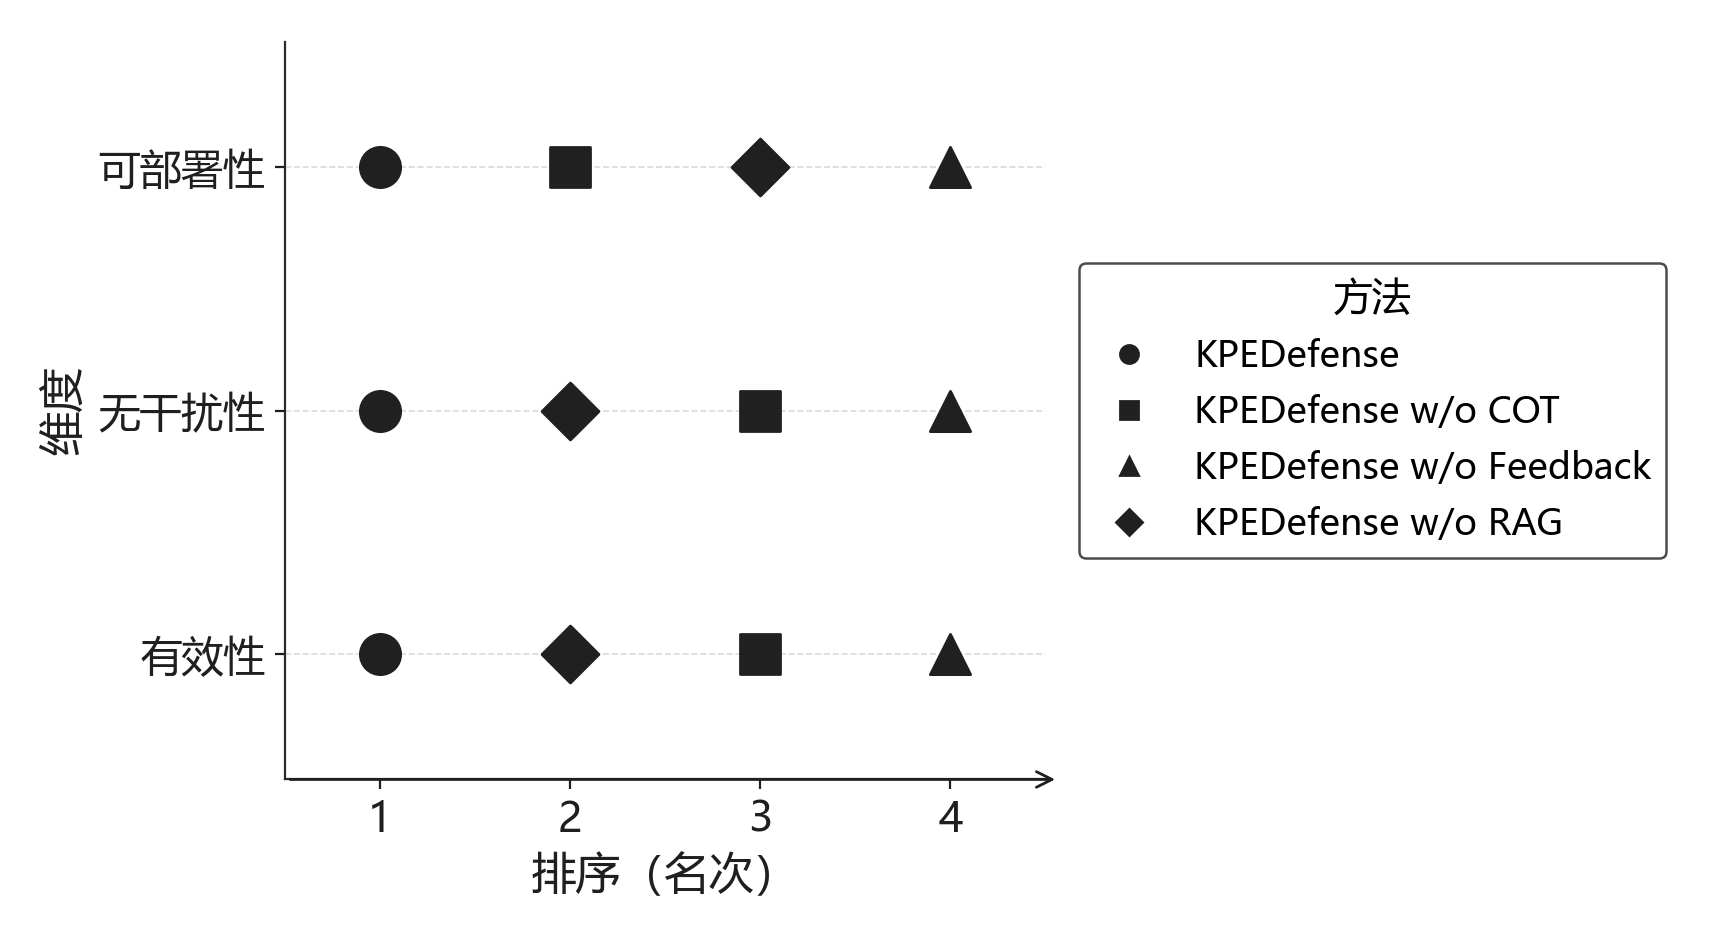
\includegraphics[width=0.85\textwidth]{images/output_rank_order/method_rank_order.png}}
	\caption{方法配置在三个维度上的排名对比。}\label{fig:method-ranking-overview}
\end{figure}

从图中可见，完整工作流 \texttt{all} 在三个维度上均排名第一（综合平均排名 $1.00$），显著优于任何消融配置。表\ref{tab:ablation-scores}给出了四种方法配置在三个维度上的详细得分。

\begin{table}[htb]
	\centering
	\bicaption{消融实验中各方法配置在三维度上的平均得分}{Average scores of method configurations across three dimensions in ablation study}
	\label{tab:ablation-scores}
	\setlength{\tabcolsep}{10pt}
	\renewcommand{\arraystretch}{1.3}
	\begin{tabularx}{0.75\linewidth}{>{\ttfamily\raggedright\arraybackslash}p{0.22\linewidth} *{3}{>{\centering\arraybackslash}X}}
	\toprule
	\textbf{方法配置} & \textbf{有效性($E$)} & \textbf{无干扰性($I$)} & \textbf{可部署性($D$)} \\
	\midrule
	all & 0.581 & 0.431 & 0.403 \\
	w/o rag & 0.476 & 0.370 & 0.321 \\
	w/o cot & 0.234 & 0.340 & 0.398 \\
	w/o feedback & 0.121 & 0.269 & 0.288 \\
	\bottomrule
	\end{tabularx}
\end{table}

\textbf{反馈迭代机制（Feedback）的核心作用：}移除反馈优化后，策略质量全面下降，三个维度得分分别为：$E=0.121$（下降79.2\%）、$I=0.269$（下降37.6\%）、$D=0.288$（下降28.5\%）。这表明迭代优化是工作流的核心环节，评审模型的多轮反馈能够持续引导生成模型修正缺陷，对有效性的提升尤为显著。

\textbf{检索增强（RAG）的知识支撑：}\texttt{w/o rag} 在有效性维度保持次优（$E=0.476$），显著优于 \texttt{w/o cot}（$E=0.234$）和 \texttt{w/o feedback}（$E=0.121$）。这说明检索增强模块为策略生成提供了关键的领域知识支撑，包括漏洞特征库、历史防控案例与Kubernetes安全最佳实践。在缺乏这些知识的情况下，生成模型更易产生不精确或不相关的策略。

\textbf{思维链推导（CoT）的双刃剑效应：}\texttt{w/o cot} 在有效性维度排名最低（$E=0.234$），但在可部署性维度接近完整工作流（$D=0.398$ vs. $D=0.403$）。这揭示了思维链推导的双重作用：虽能显著提升策略的漏洞覆盖率与防控逻辑严密性，但分阶段推导过程引入了更复杂的YAML配置结构与依赖关系，增加了部署门槛。在对安全性要求极高的场景下，应优先保留CoT模块；而在快速响应场景下，可适当简化推导过程以降低部署复杂度。

综上，三个模块的协同作用为策略生成提供了一致性增益，其重要性排序为：\textbf{Feedback > RAG > CoT}。完整工作流在三个维度上分别达到0.581（有效性）、0.431（无干扰性）与0.403（可部署性）的最优表现。在实际部署中，若资源受限需简化工作流，建议优先保留反馈迭代机制与检索增强模块。

\subsection{工作流跨模型稳健性验证}

为验证上述消融实验结论是否对不同生成模型稳健，本小节分析完整工作流相对消融配置的优势在不同模型条件下的一致性。

图\ref{fig:effectiveness-profile-avg} 给出不同生成模型在有效性维度的平均排名。图\ref{fig:effectiveness-generator-by-method} 与图\ref{fig:effectiveness-generator-grouped} 从生成模型视角展开方法配置贡献结构。

\begin{figure}[!ht]
	\centering
	{\setlength{\abovecaptionskip}{2pt}%
	 \setlength{\belowcaptionskip}{0pt}%
	 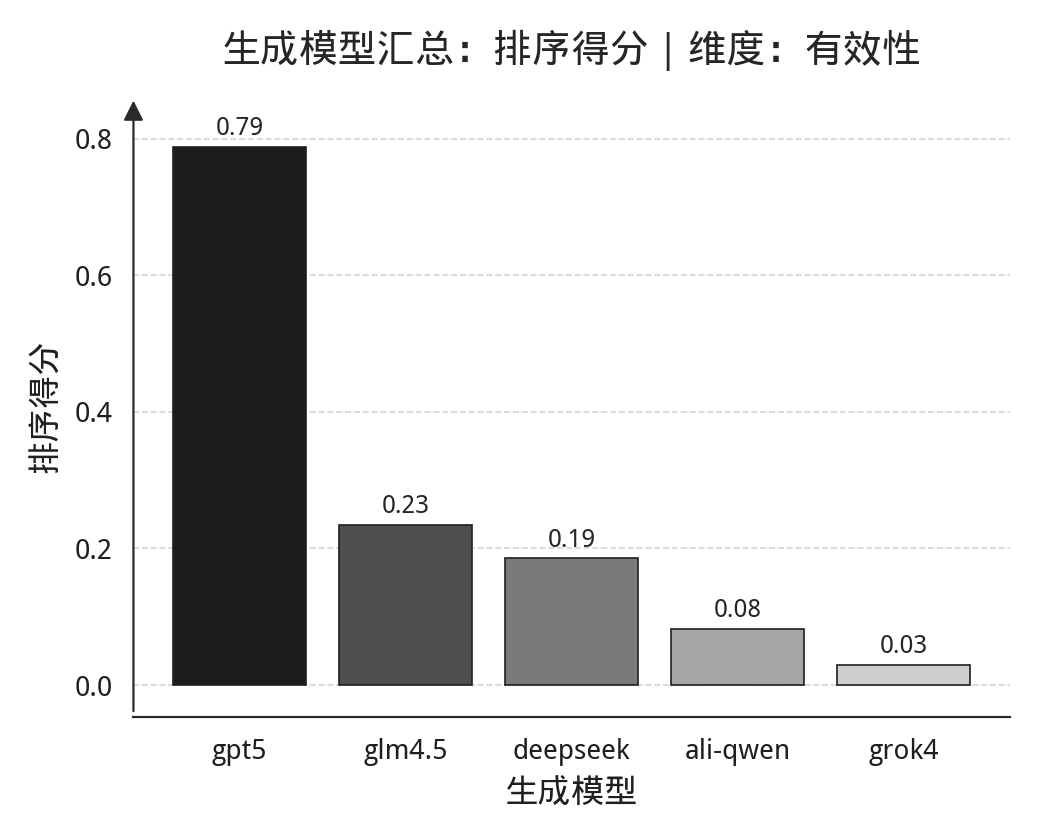
\includegraphics[width=0.85\textwidth]{images/plots/有效性/summary/single_dim_profile_avg_有效性.png}}
	\caption{有效性维度下，不同生成模型的平均排名式评分结果（跨评审者汇总）。}\label{fig:effectiveness-profile-avg}
\end{figure}

\begin{figure}[!ht]
	\centering
	{\setlength{\abovecaptionskip}{2pt}%
	 \setlength{\belowcaptionskip}{0pt}%
	 \subfloat[\texttt{Qwen3}\label{fig:effectiveness-generator-by-method-qwen3}]{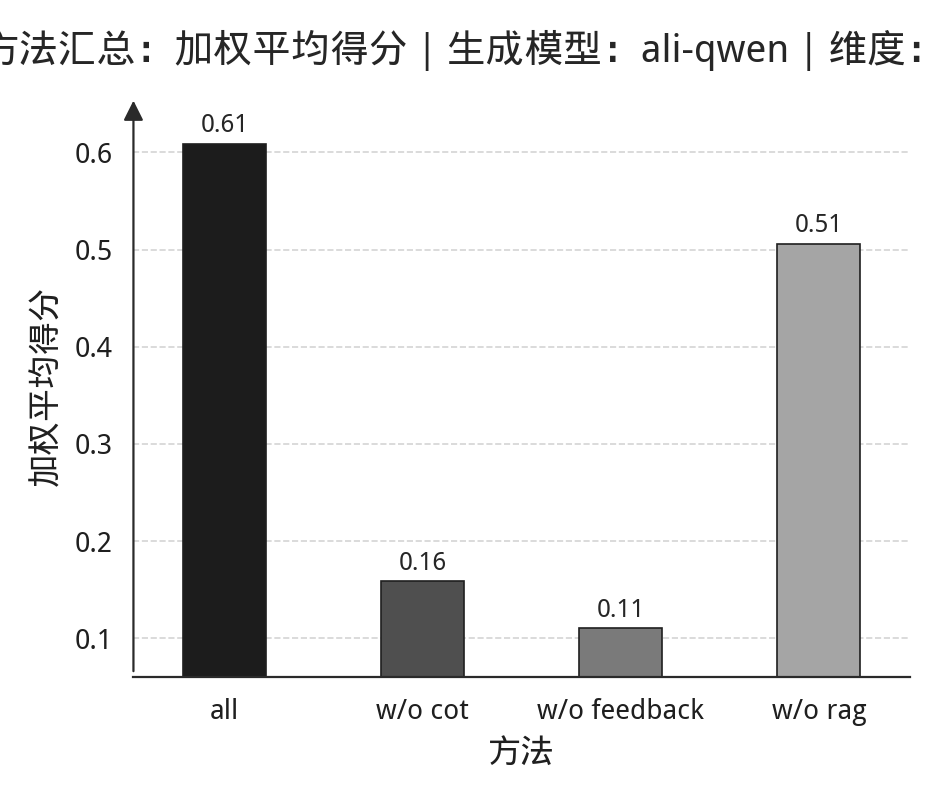
\includegraphics[width=0.32\textwidth]{images/plots/有效性/generator/ali-qwen/generator_bar_by_method_ali-qwen_有效性.png}}\hfill
	 \subfloat[\texttt{DeepSeek}\label{fig:effectiveness-generator-by-method-deepseek}]{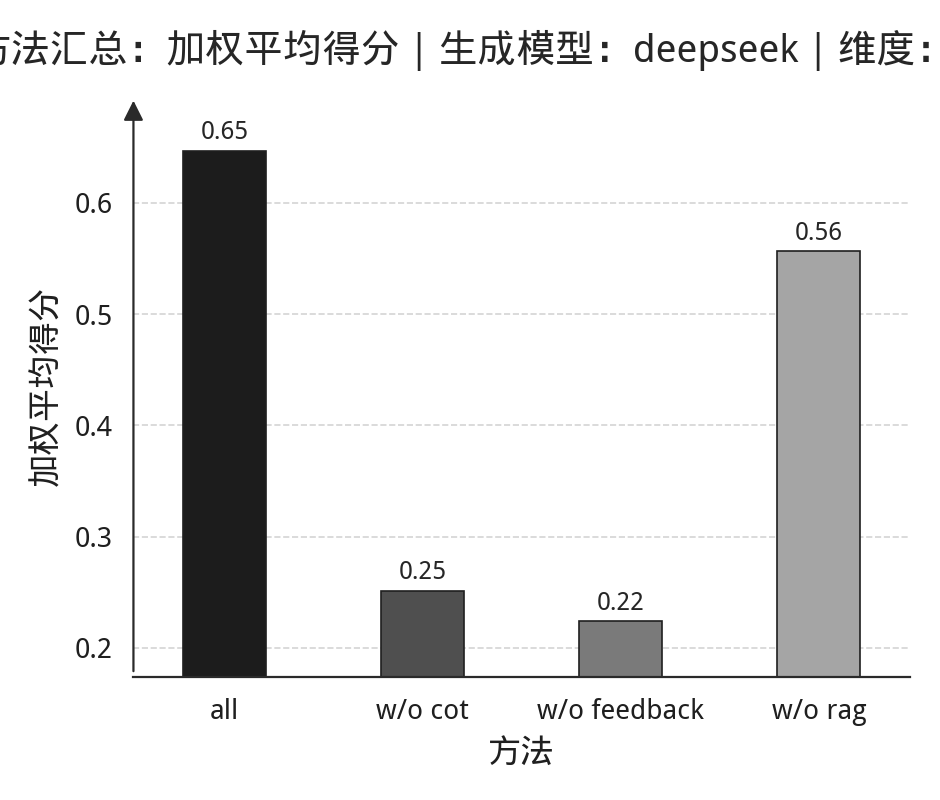
\includegraphics[width=0.32\textwidth]{images/plots/有效性/generator/deepseek/generator_bar_by_method_deepseek_有效性.png}}\hfill
	 \subfloat[\texttt{GPT-5}\label{fig:effectiveness-generator-by-method-gpt5}]{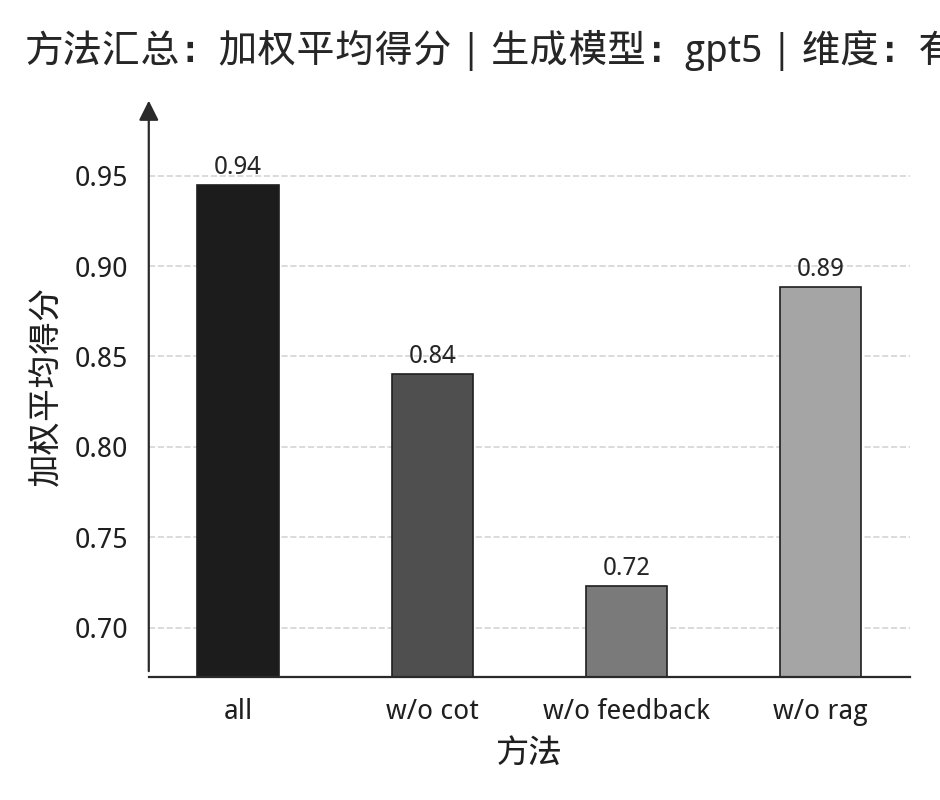
\includegraphics[width=0.32\textwidth]{images/plots/有效性/generator/gpt5/generator_bar_by_method_gpt5_有效性.png}}\\
	 \subfloat[\texttt{Grok}\label{fig:effectiveness-generator-by-method-grok}]{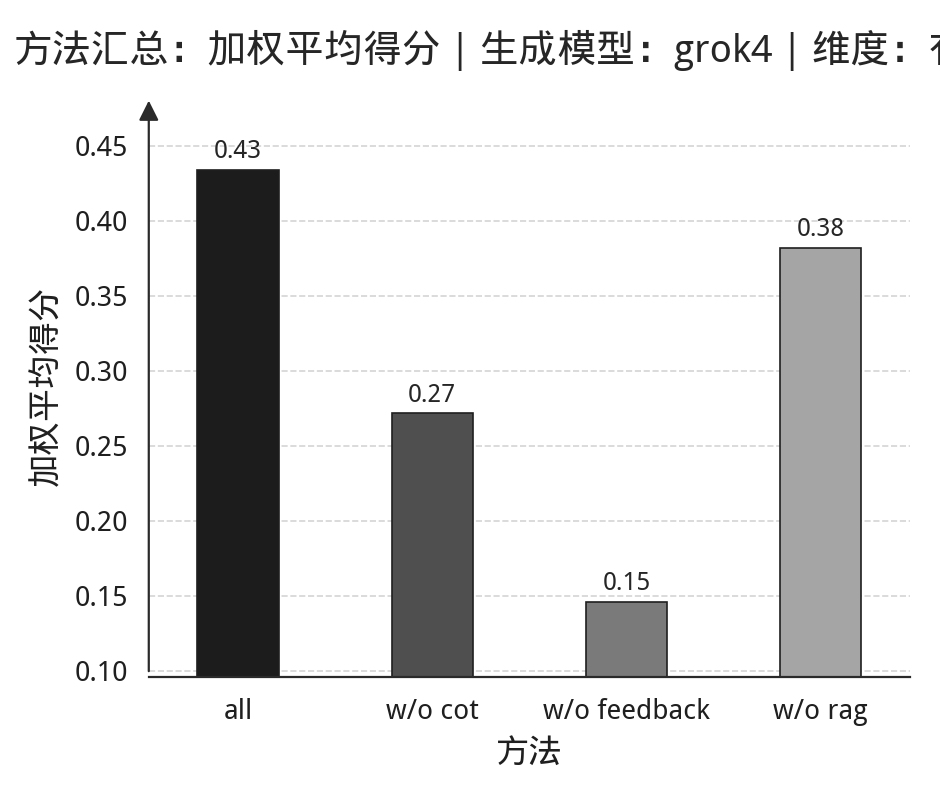
\includegraphics[width=0.32\textwidth]{images/plots/有效性/generator/grok4/generator_bar_by_method_grok4_有效性.png}}\hfill
	 \subfloat[\texttt{GLM-4.6}\label{fig:effectiveness-generator-by-method-glm46}]{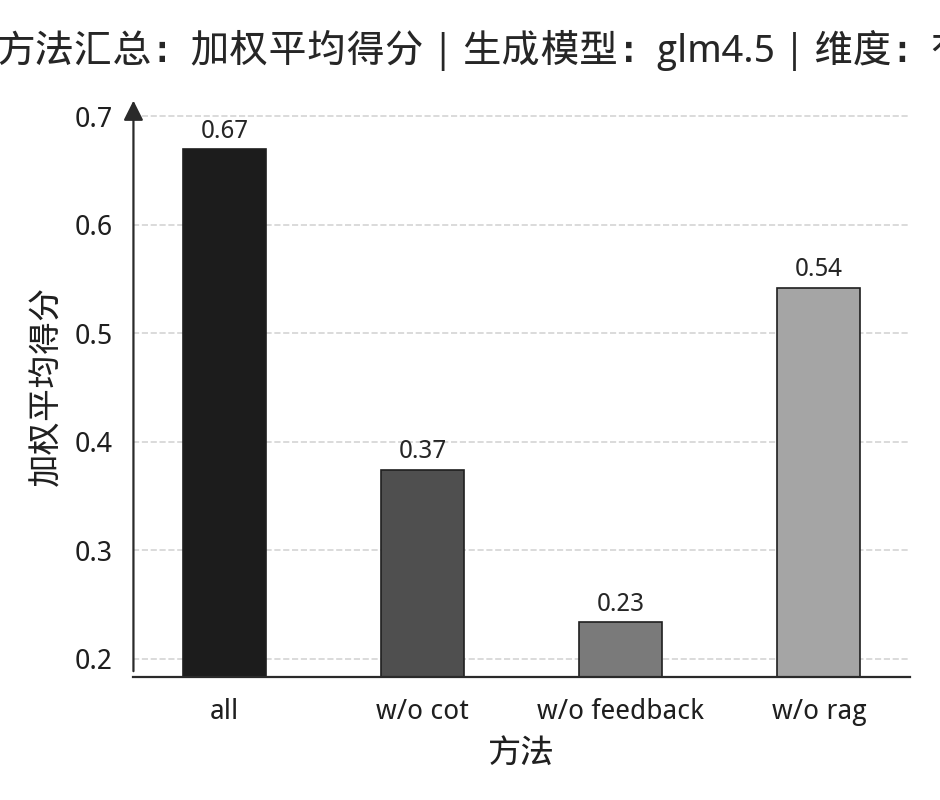
\includegraphics[width=0.32\textwidth]{images/plots/有效性/generator/glm4.5/generator_bar_by_method_glm4.5_有效性.png}}}
	\caption{有效性维度下，不同生成模型的工作流贡献结构对照（3+2 网格）。}\label{fig:effectiveness-generator-by-method}
\end{figure}

\begin{figure}[!ht]
	\centering
	{\setlength{\abovecaptionskip}{2pt}%
	 \setlength{\belowcaptionskip}{0pt}%
	 \subfloat[\texttt{Qwen3}\label{fig:effectiveness-generator-grouped-qwen3}]{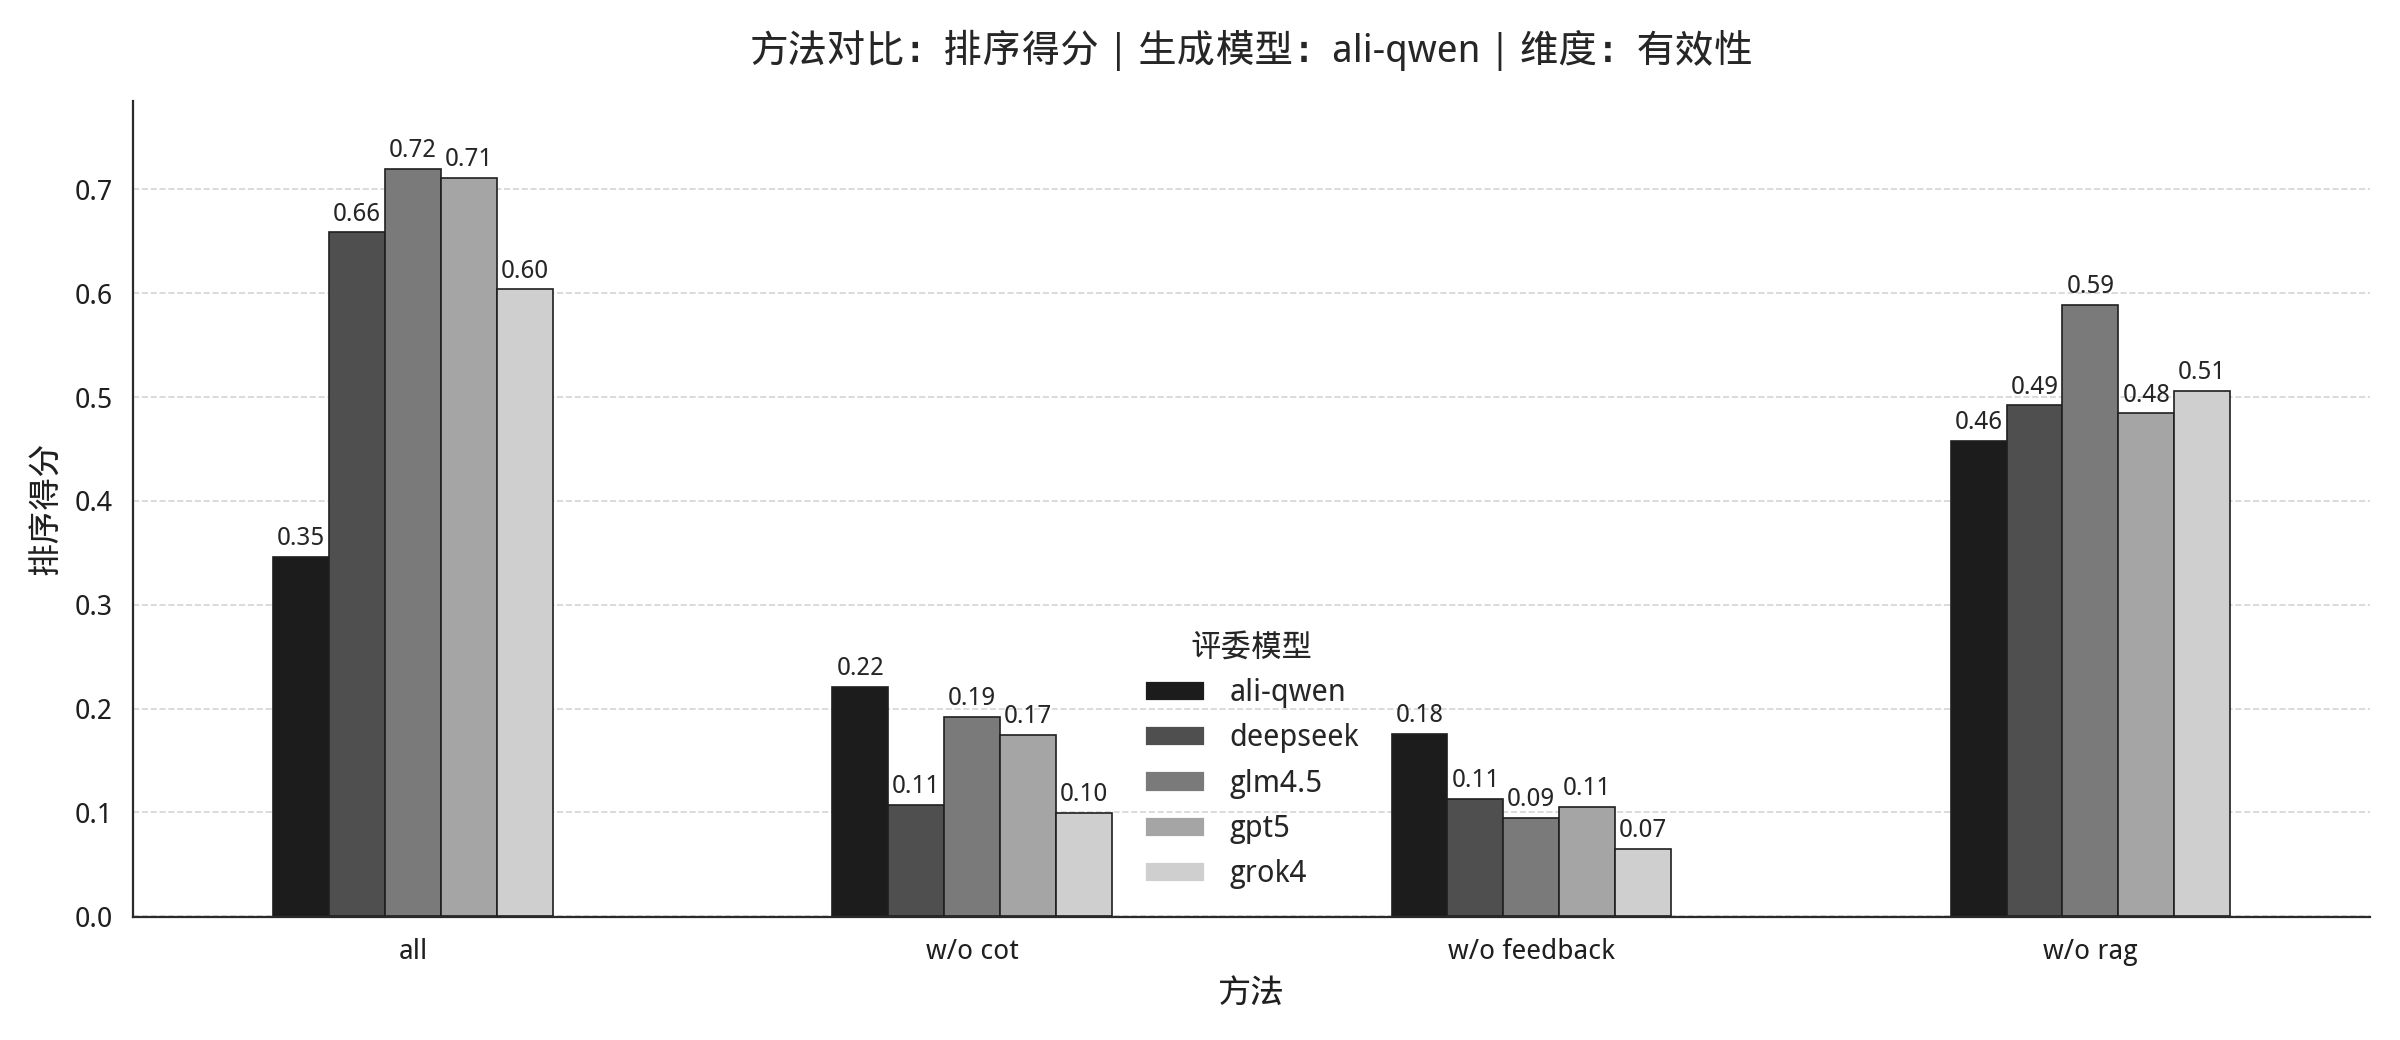
\includegraphics[width=0.32\textwidth]{images/plots/有效性/generator/ali-qwen/grouped_bar_ali-qwen_有效性.png}}\hfill
	 \subfloat[\texttt{DeepSeek}\label{fig:effectiveness-generator-grouped-deepseek}]{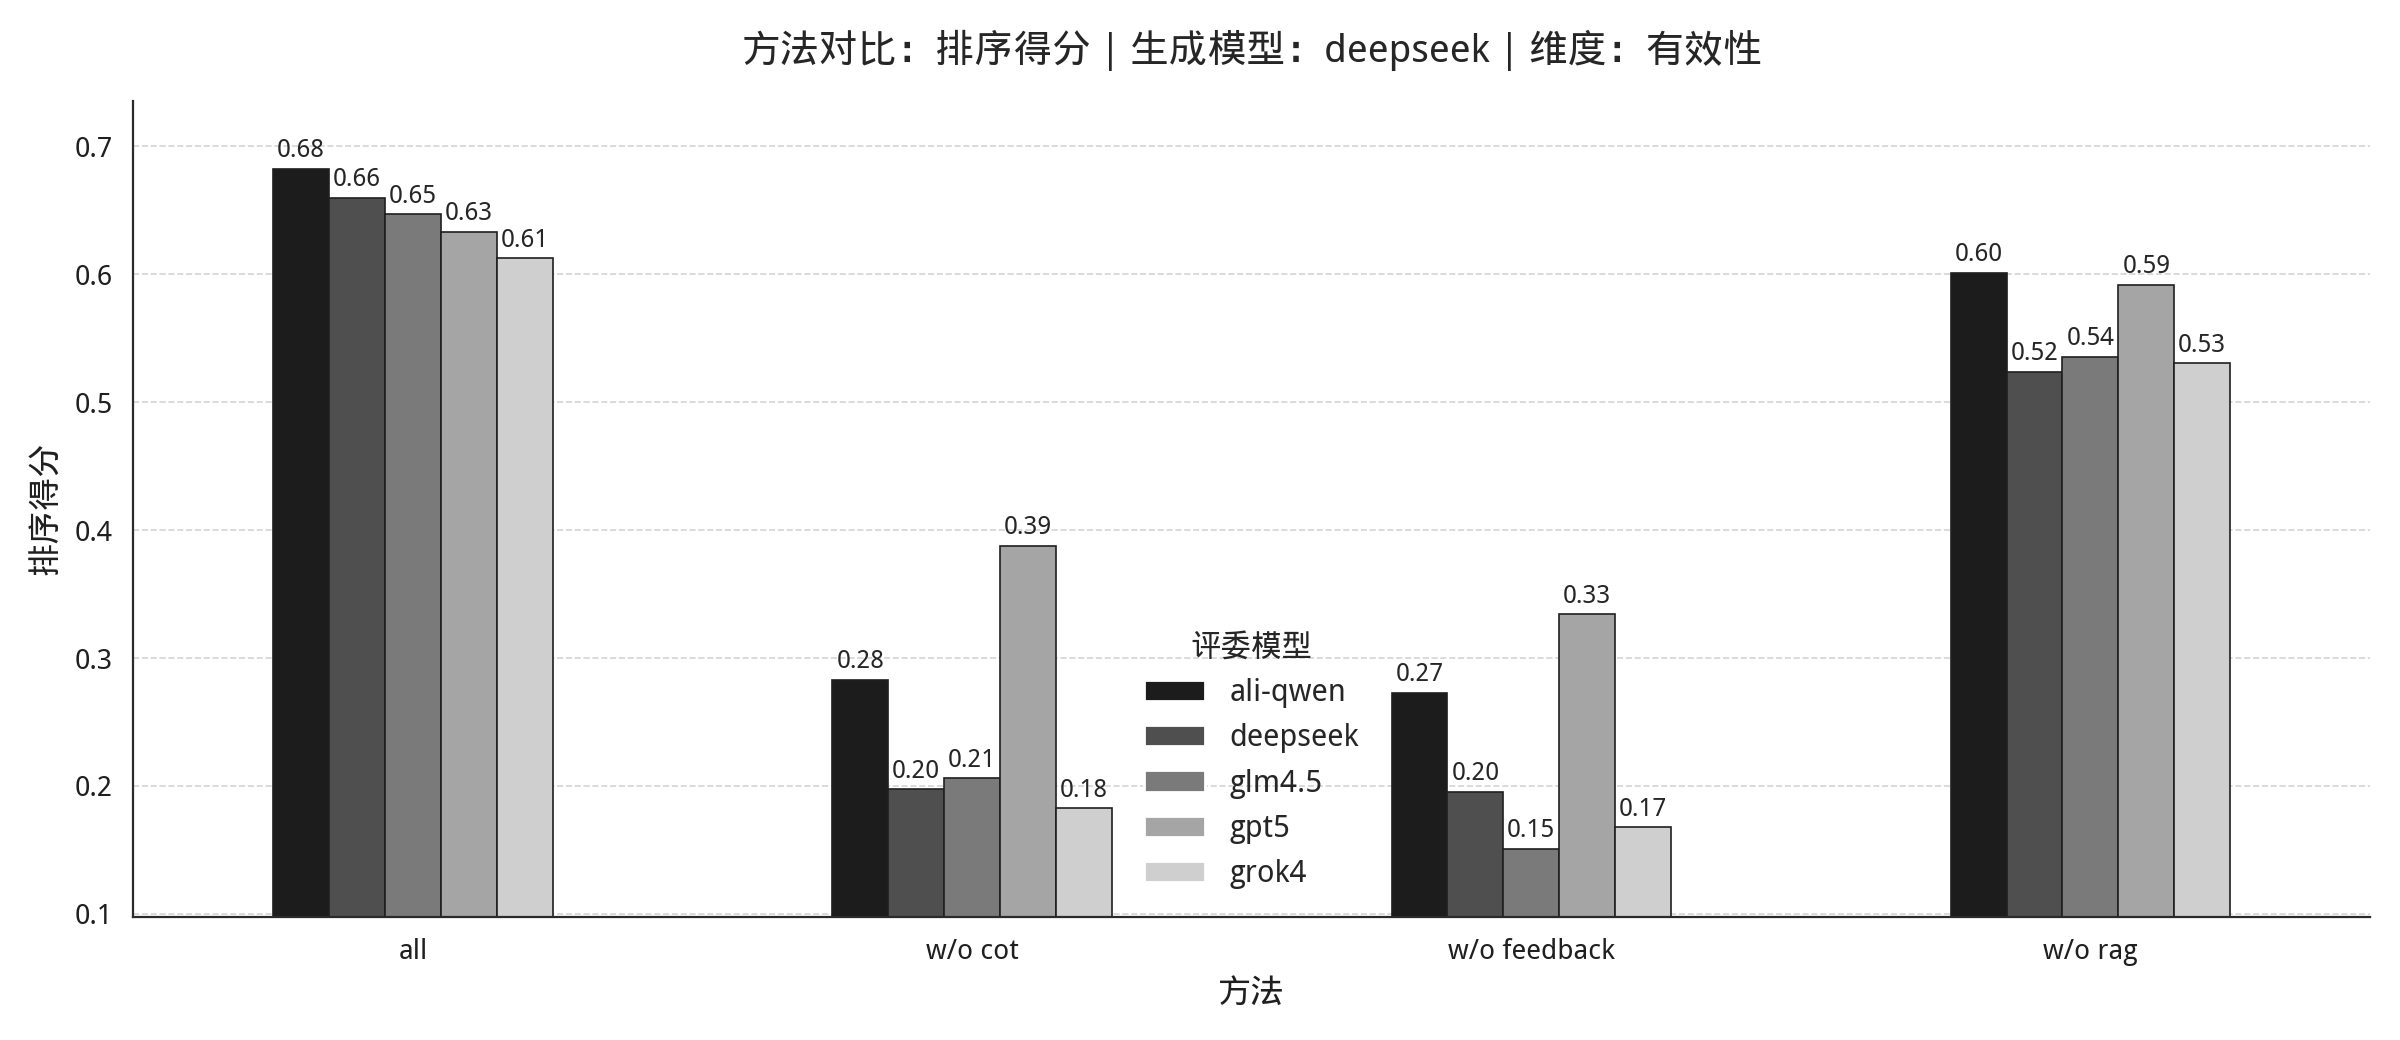
\includegraphics[width=0.32\textwidth]{images/plots/有效性/generator/deepseek/grouped_bar_deepseek_有效性.png}}\hfill
	 \subfloat[\texttt{GPT-5}\label{fig:effectiveness-generator-grouped-gpt5}]{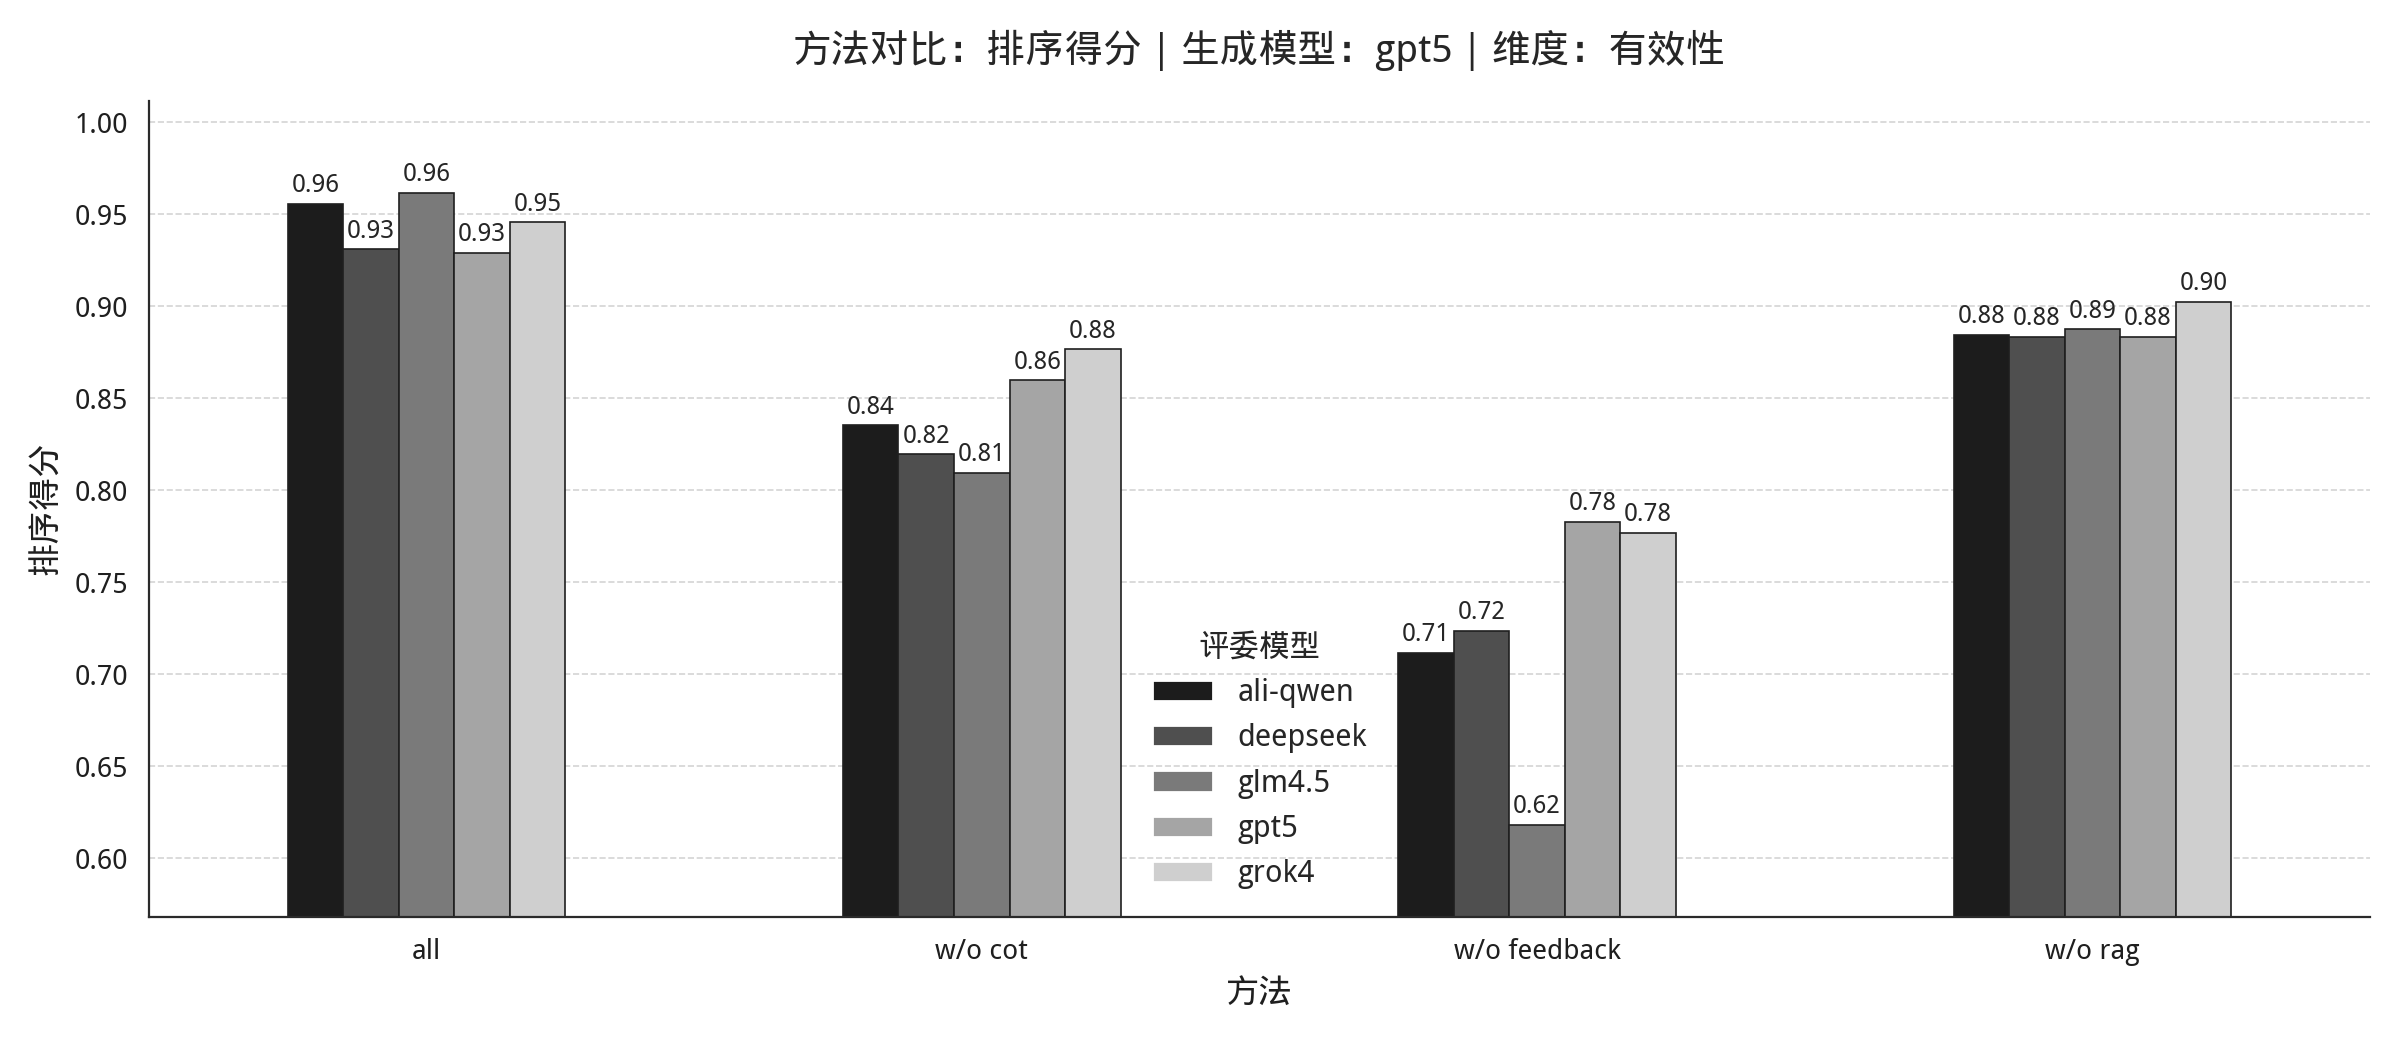
\includegraphics[width=0.32\textwidth]{images/plots/有效性/generator/gpt5/grouped_bar_gpt5_有效性.png}}\\
	 \subfloat[\texttt{Grok}\label{fig:effectiveness-generator-grouped-grok}]{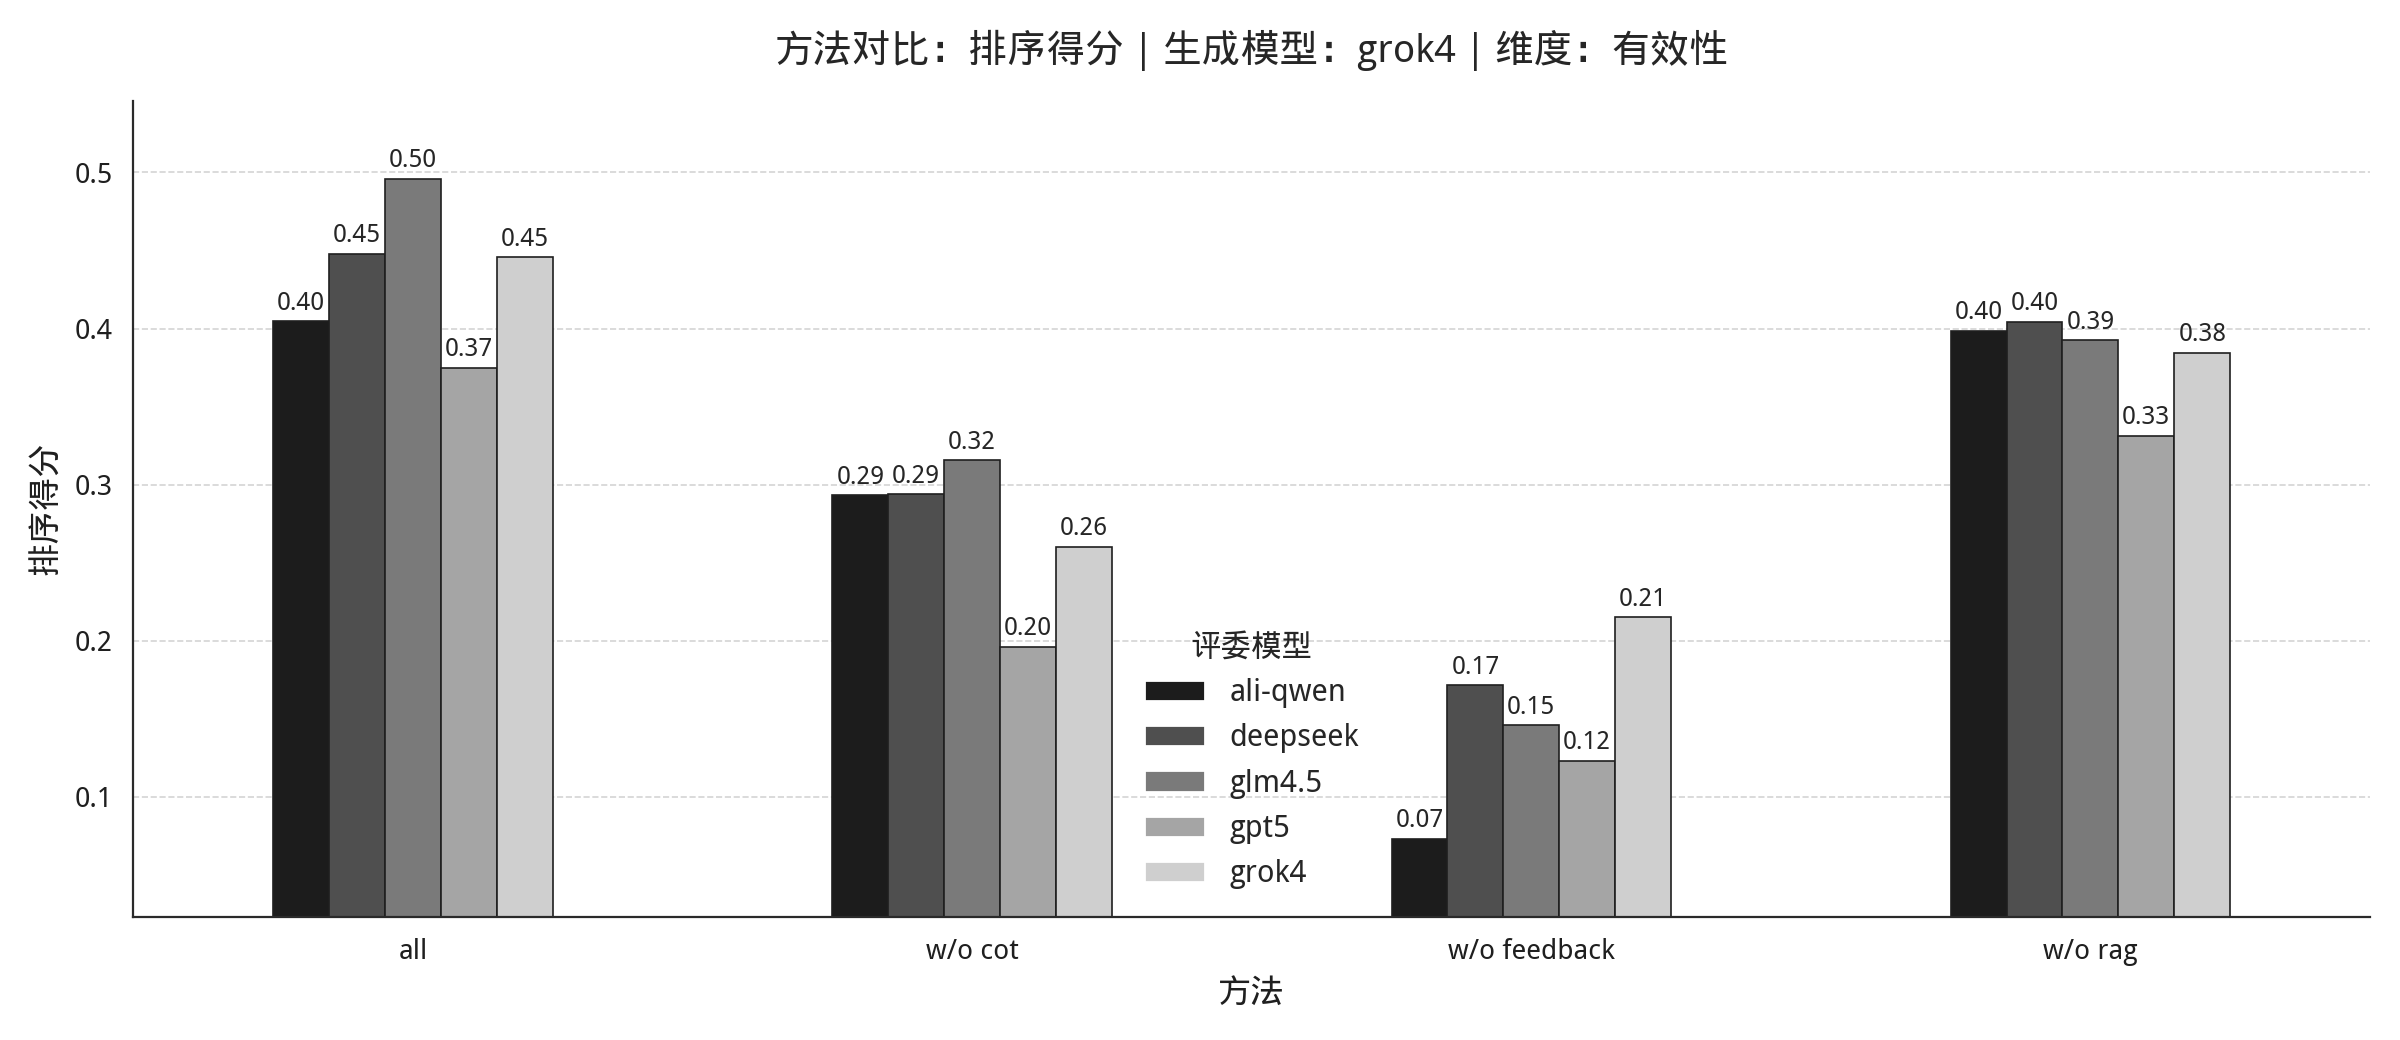
\includegraphics[width=0.32\textwidth]{images/plots/有效性/generator/grok4/grouped_bar_grok4_有效性.png}}\hfill
	 \subfloat[\texttt{GLM-4.6}\label{fig:effectiveness-generator-grouped-glm46}]{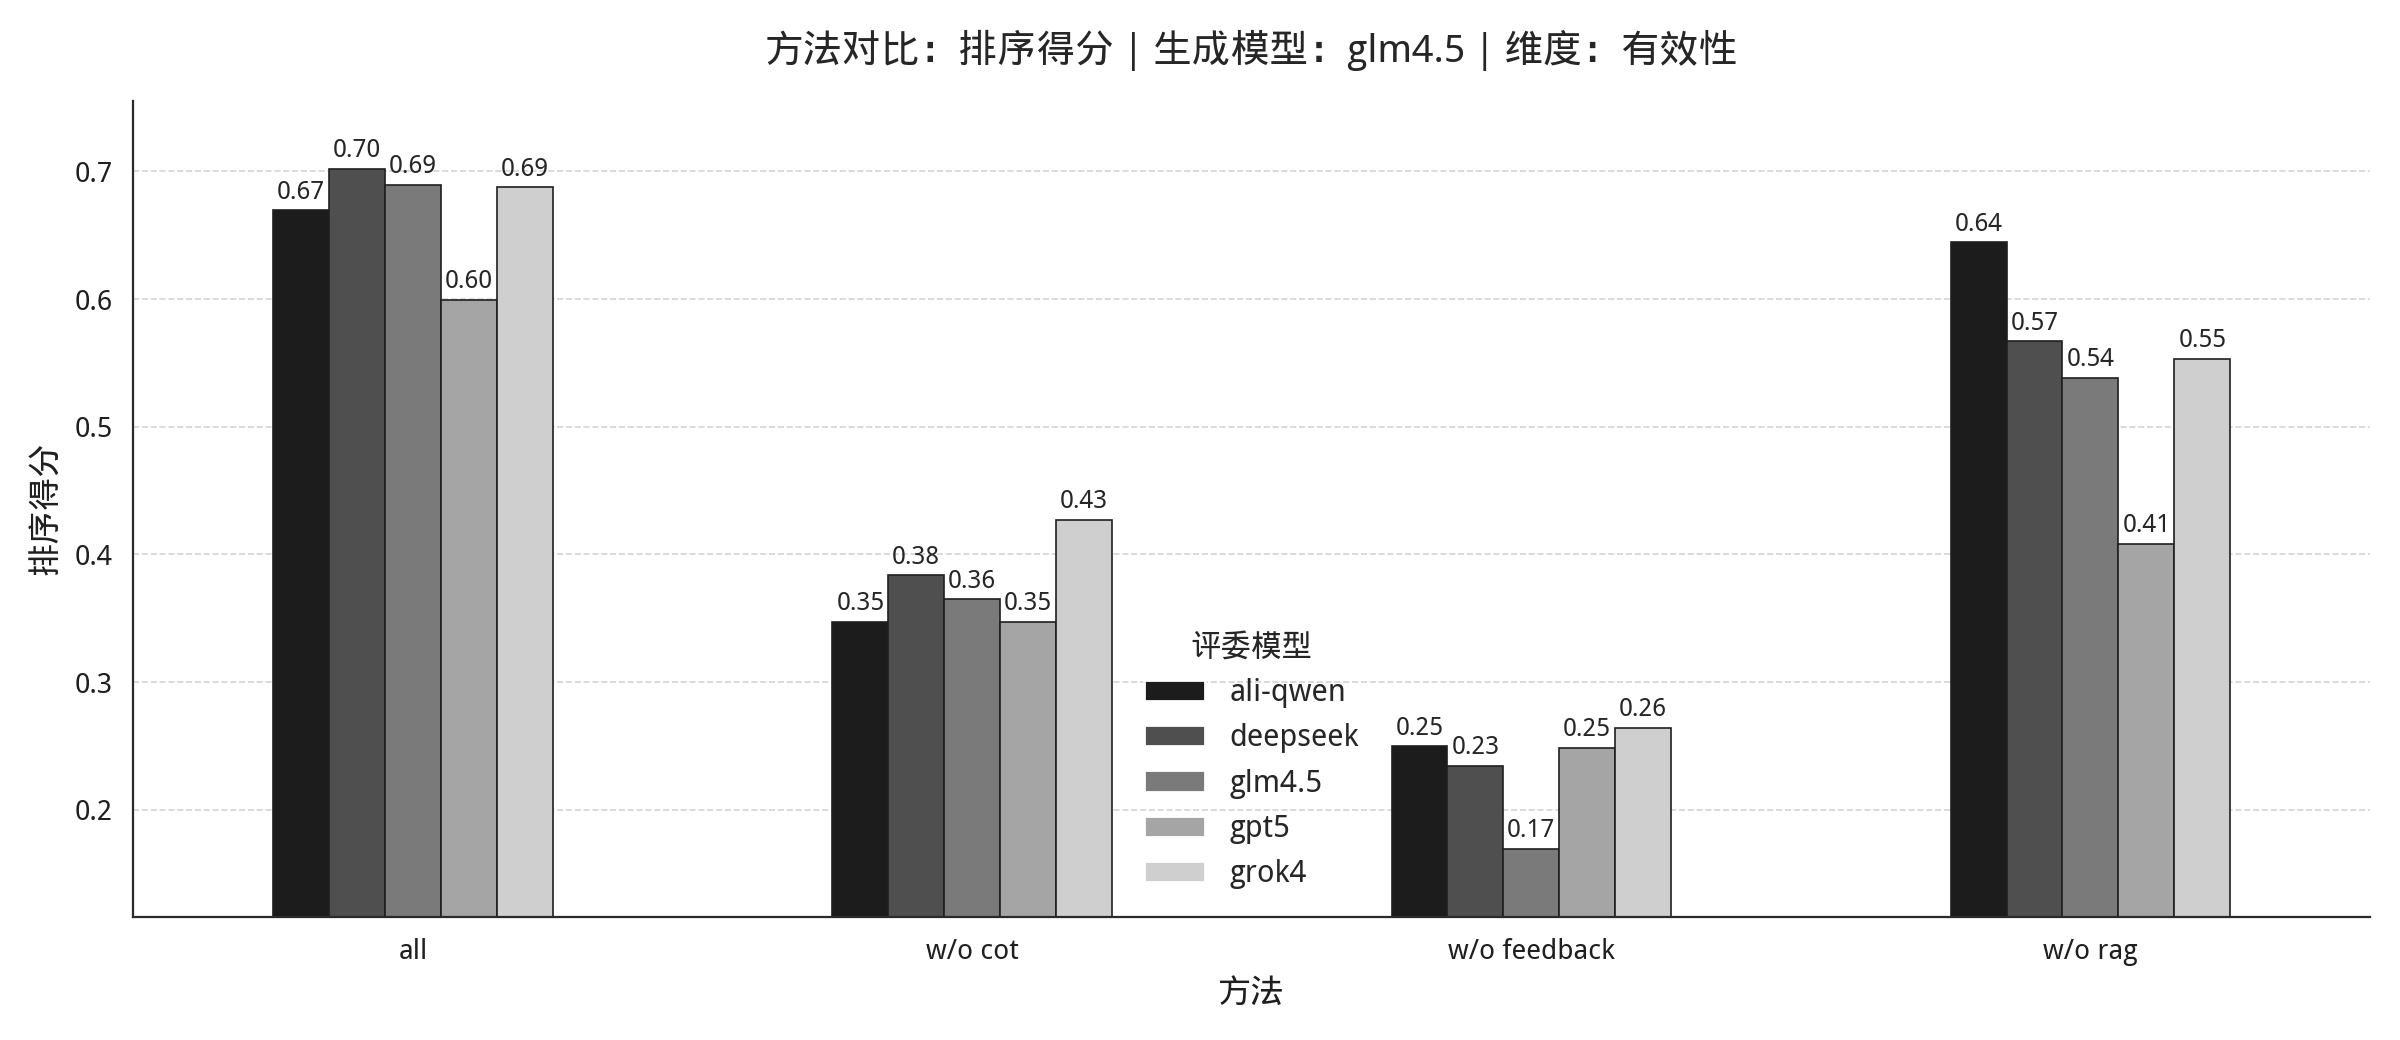
\includegraphics[width=0.32\textwidth]{images/plots/有效性/generator/glm4.5/grouped_bar_glm4.5_有效性.png}}}
	\caption{有效性维度下，不同生成模型的分组条形图对照（3+2 网格）。}\label{fig:effectiveness-generator-grouped}
\end{figure}

从图中可见，完整工作流（\texttt{all}）在五个生成模型条件下均保持最优或次优排名，验证了消融实验结论的跨模型稳健性。不同生成模型对各模块的依赖程度存在差异：GPT-5 与 GLM-4.5 对反馈迭代的依赖性更强，移除反馈后排名下降明显；而 DeepSeek 与 Qwen3 对检索增强的响应更为敏感，说明不同模型在知识库支撑与迭代优化上的需求存在差异。

\section{RQ2：生成模型能力评估}

本节从策略生成质量与输出稳定性两个维度评估五个生成模型的能力特征，识别不同模型在三维质量指标上的取舍倾向与适用场景。

\subsection{三维质量指标的能力分化}

图\ref{fig:generator-ranking-overview}展示了五个生成模型在有效性（$E$）、无干扰性（$I$）与可部署性（$D$）三个维度上的排名分布。

\begin{figure}[!ht]
	\centering
	{\setlength{\abovecaptionskip}{2pt}%
	 \setlength{\belowcaptionskip}{0pt}%
	 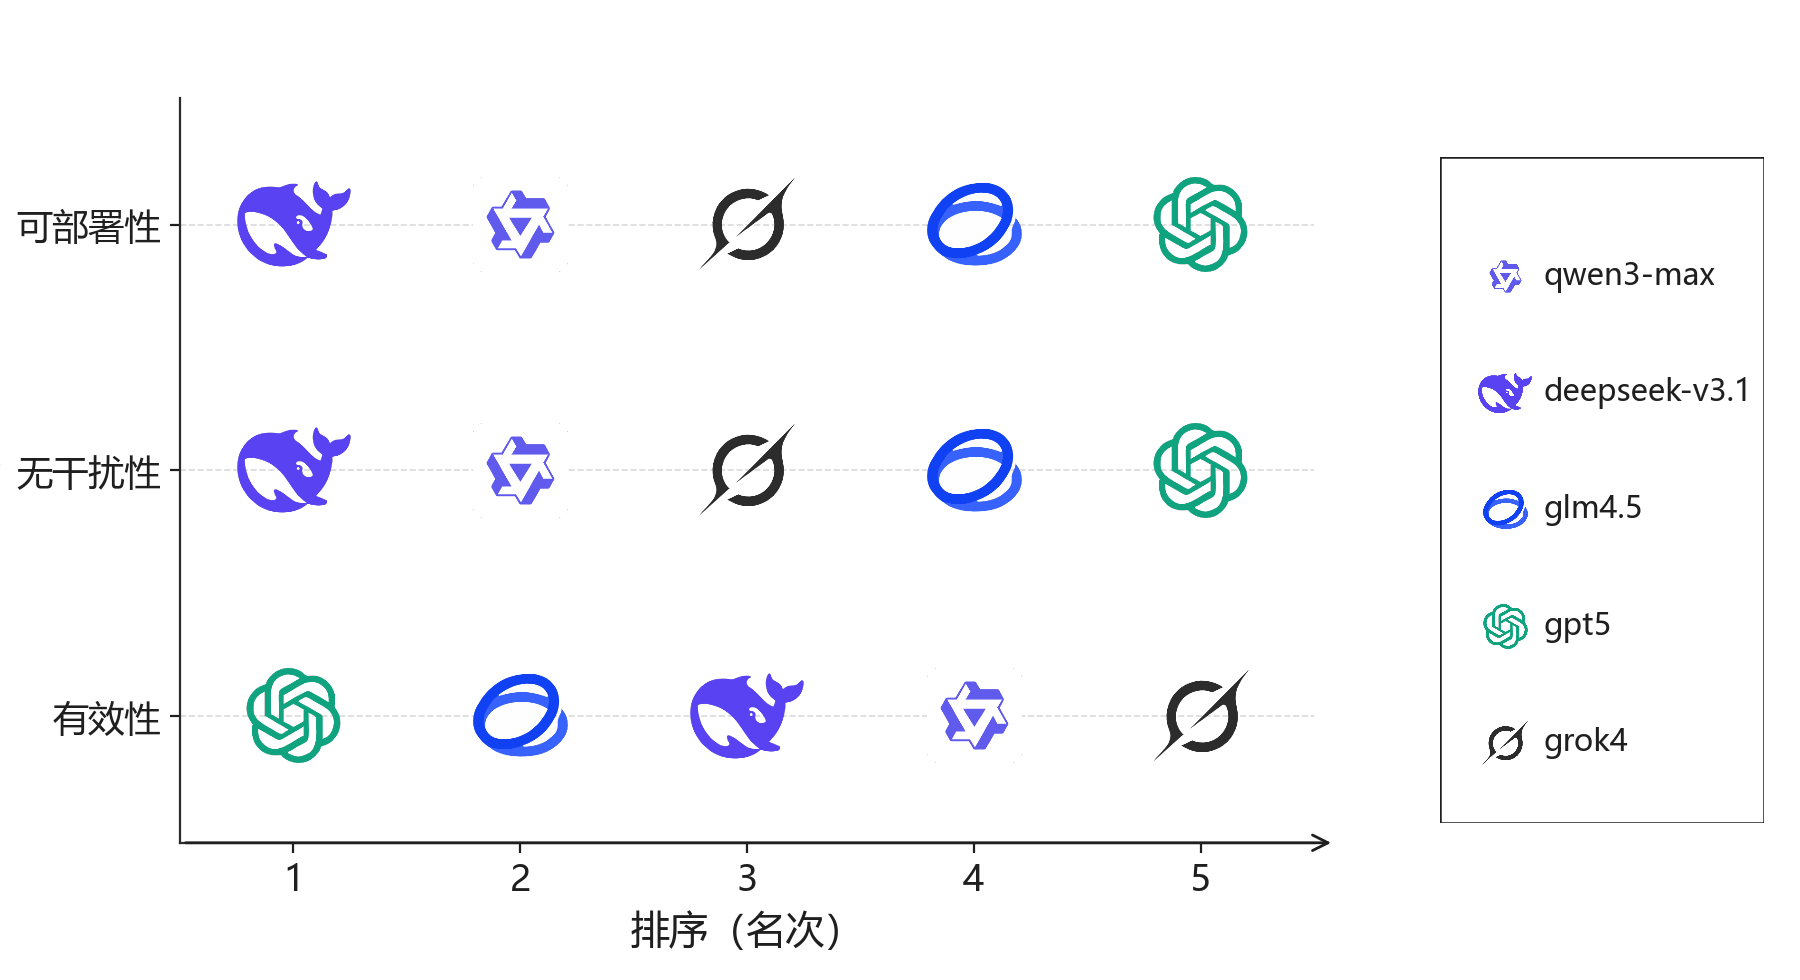
\includegraphics[width=0.85\textwidth]{images/output_rank_order/profile_rank_order.png}}
	\caption{生成模型在三个维度上的排名对比。}\label{fig:generator-ranking-overview}
\end{figure}

表\ref{tab:generator-scores}给出了五个生成模型在三个维度上的详细得分，揭示了显著的能力分化现象。

\begin{table}[htb]
	\centering
	\bicaption{生成模型在三维度上的平均得分}{Average scores of generation models across three dimensions}
	\label{tab:generator-scores}
	\setlength{\tabcolsep}{8pt}
	\renewcommand{\arraystretch}{1.3}
	\begin{tabularx}{0.85\linewidth}{>{\ttfamily\raggedright\arraybackslash}p{0.20\linewidth} *{3}{>{\centering\arraybackslash}X} >{\centering\arraybackslash}p{0.15\linewidth}}
	\toprule
	\textbf{生成模型} & \textbf{有效性($E$)} & \textbf{无干扰性($I$)} & \textbf{可部署性($D$)} & \textbf{综合评价} \\
	\midrule
	GPT-5 & \textbf{0.814} & 0.175 & 0.000 & 安全优先型 \\
	GLM-4.5 & 0.327 & 0.324 & 0.336 & 中等均衡型 \\
	DeepSeek & 0.284 & \textbf{0.497} & \textbf{0.605} & 部署优先型 \\
	Qwen3-Max & 0.193 & 0.425 & 0.477 & 稳定通用型 \\
	Grok4 & 0.147 & 0.342 & 0.346 & 轻量快速型 \\
	\bottomrule
	\end{tabularx}
\end{table}

\textbf{DeepSeek 3.1：部署优先型优选方案。}\texttt{DeepSeek 3.1} 在可部署性与无干扰性维度表现卓越（$D=0.605$，$I=0.497$），均位列首位，但在有效性维度处于中游（$E=0.284$）。这表明 DeepSeek 擅长生成简洁、低侵入性的策略，能够有效平衡漏洞防控与实际部署约束，规避过度复杂的配置设计。该特性使其成为对部署速度与业务连续性敏感的生产环境的首选方案，尤其适用于需要快速响应新披露漏洞的场景。

\textbf{GPT-5：安全优先型方案。}\texttt{GPT-5} 呈现极端的维度分化特征：在有效性维度遥遥领先（$E=0.814$），但在无干扰性与可部署性维度排名垫底（$I=0.175$，$D=0.000$）。这一分化现象揭示 GPT-5 在生成策略时极度注重漏洞防控的彻底性，倾向于采用严格的RBAC限制、网络隔离与准入控制措施，不惜牺牲策略的简洁性与部署便利性。该模型适用于对安全性要求极高且可容忍高部署成本的关键基础设施场景，如金融、政务等领域的Kubernetes集群防护。

\textbf{Qwen3-Max：稳定通用型方案。}\texttt{Qwen3-Max} 在三维度上保持中上水平（$E=0.193$，$I=0.425$，$D=0.477$），无明显短板，呈现较为均衡的能力分布。虽未在任何单一维度上拔尖，但其稳定性使其可作为通用型选择，适用于对三个维度均有一定要求且需要平衡多目标的场景。

\textbf{GLM-4.5：中等均衡型方案。}\texttt{GLM-4.5} 在三个维度上得分接近（$E=0.327$，$I=0.324$，$D=0.336$），表现出良好的均衡性，但整体水平处于中游。其维度分化程度较小，适合作为多模型组合策略中的补充选择。

\textbf{Grok4：轻量快速型方案。}\texttt{Grok4} 在有效性维度排名最低（$E=0.147$），但在无干扰性与可部署性维度保持中游水平（$I=0.342$，$D=0.346$）。这表明 Grok4 倾向于生成简单、轻量级的策略，虽然防控效果有限，但部署门槛低、响应速度快，适用于低风险漏洞的临时防控或作为快速应急响应方案。

\subsection{输出稳定性评估}

为评估不同生成模型在策略生成过程中的输出稳定性，本文统计了各模型在生成阶段触发重试的次数。重试机制主要针对三类失败情形：结构化输出的 JSON 格式错误（通常因字段缺失、括号不匹配或编码问题）、生成内容的语法错误（包括 YAML 语法错误、逻辑矛盾或不可解析的配置片段），以及内容违规（触发模型供应商的安全策略或内容审核机制）。为便于跨模型对比，本文将计数按固定分母 504 归一化为失误率。表\ref{tab:model-retry-stats} 给出五个生成模型的失误率统计（=计数/504）。

\begin{table}[htb]
	\centering
	\bicaption{生成模型在策略生成过程中的重试失误率（\%）统计（=计数/504）}{Failure rates (\%) of retry-triggering errors during strategy generation across LLMs (=count/504)}
    \label{tab:model-retry-stats}
	\setlength{\tabcolsep}{8pt}
	\renewcommand{\arraystretch}{1.2}
	\small
	\begin{tabularx}{0.95\linewidth}{>{\raggedright\arraybackslash}p{2.6cm} *{5}{>{\centering\arraybackslash}X}}
    \toprule
	\textbf{错误类型} & \makecell{\textbf{DeepSeek}\\\textbf{3.1}} & \makecell{\textbf{GLM}\\\textbf{-4.5}} & \makecell{\textbf{GPT}\\\textbf{-5}} & \makecell{\textbf{Grok}\\\textbf{4}} & \makecell{\textbf{Qwen}\\\textbf{3}} \\
    \midrule
	JSON 格式错误 & 0.99\% & 4.56\% & 0.00\% & 0.99\% & 2.58\% \\
	语法错误 & 0.60\% & 1.98\% & 0.00\% & 0.00\% & 0.99\% \\
	内容违规 & 0.00\% & 1.98\% & 0.00\% & 0.00\% & 0.00\% \\
	\addlinespace[0.25em]\midrule
	\textbf{合计} & \textbf{1.59\%} & \textbf{8.53\%} & \textbf{0.00\%} & \textbf{0.99\%} & \textbf{3.57\%} \\
    \bottomrule
	\end{tabularx}
\end{table}

整体上，GPT-5 在三类错误上均无重试记录，表现出较高的生成鲁棒性；Grok 和 DeepSeek 的失误率较低，输出稳定性良好；Qwen3 与 GLM-4.5 的失误率相对较高，尤其在 JSON 格式错误上，GLM-4.5 的失误率为 4.56\%（=23/504），反映其在结构化输出约束下的遵循能力有待提升。语法错误维度上，GLM-4.5 同样表现出明显劣势（1.98\%=10/504），而其余模型均不超过 0.99\%（=5/504）。值得注意的是，GLM-4.5 是唯一触发内容违规的模型（1.98\%=10/504），可能与其内容审核策略对高危漏洞描述中的安全关键词过度敏感相关。

该统计为模型选型与多智能体协同策略提供了量化参考：在资源受限或对输出稳定性敏感的场景下，优先选用 GPT-5、Grok 或 DeepSeek；而对于需要多样性候选集的场景，可将 Qwen3 与 GLM-4.5 纳入候选池，但需配置更宽松的重试预算与后处理容错机制。

\subsection{生成模型能力评估小结}

五个生成模型在三维质量指标上表征出明显的能力分化与取舍倾向：DeepSeek 的部署优势（$D=0.605$）使其成为生产环境首选；GPT-5 的安全优势（$E=0.814$）适用于高安全要求场景；Grok4 可作为快速响应的轻量级方案（$D=0.346$，响应时间最短）。

进一步分析各生成模型的最佳方法配置（表\ref{tab:best-method-per-generator}）发现，所有模型在完整工作流（\texttt{all}）配置下均达到最优或次优表现，验证了RQ1消融实验结论的跨模型稳健性。值得注意的是，DeepSeek 在 \texttt{w/o cot} 配置下的可部署性得分达到0.749，超过完整工作流的0.678，进一步证实了思维链推导在提升防控效果的同时会增加部署复杂度的双刃剑效应。

\begin{table}[htb]
	\centering
	\bicaption{各生成模型的最佳方法配置与得分}{Best method configuration and score for each generation model}
	\label{tab:best-method-per-generator}
	\setlength{\tabcolsep}{8pt}
	\renewcommand{\arraystretch}{1.3}
	\begin{tabularx}{0.90\linewidth}{>{\ttfamily\raggedright\arraybackslash}p{0.18\linewidth} >{\centering\arraybackslash}X >{\centering\arraybackslash}X >{\centering\arraybackslash}X}
	\toprule
	\textbf{生成模型} & \textbf{有效性最佳} & \textbf{无干扰性最佳} & \textbf{可部署性最佳} \\
	\midrule
	GPT-5 & all (0.945) & w/o cot (0.369) & w/o cot (0.256) \\
	GLM-4.5 & all (0.670) & all (0.522) & all (0.504) \\
	DeepSeek & all (0.647) & w/o rag (0.634) & w/o cot (0.749) \\
	Qwen3-Max & all (0.609) & all (0.629) & all (0.656) \\
	Grok4 & all (0.434) & all (0.589) & all (0.597) \\
	\bottomrule
	\end{tabularx}
\end{table}

在输出稳定性上，GPT-5、Grok 与 DeepSeek 表现优异（失误率分别为0.00\%、0.99\%与1.59\%），而 GLM-4.5 与 Qwen3 需额外关注结构化输出约束（失误率分别为8.53\%与3.57\%）。这些实证发现为后续基于维度加权的多智能体策略组合提供了依据：在实际部署中，可依据具体漏洞的风险等级与业务约束动态选择或组合不同生成模型——对于高危漏洞优先选择GPT-5或GLM-4.5以提升防控彻底性，对于需快速部署的场景优先选择DeepSeek或Qwen3-Max以降低实施难度。

\section{RQ3：评审模型一致性评估}

为验证排名式评价的可信度，本节分析不同评审模型在单一维度与跨维度场景下的一致性，以支撑前述跨评审聚合统计与反馈闭环（RQ1--RQ2）。若不同评审者（评审模型）对候选项优劣的判断高度一致，则聚合后的排序结果更稳定、更可解释；反之，若一致性较弱，则需要警惕"评审者选择敏感性"，并进一步细化评价准则。

\subsection{跨维度的评审差异}

图\ref{fig:single-dim-by-judge-3d} 展示不同评审模型下的单维度排名式结果，反映评审模型之间的尺度差异与偏好结构。图\ref{fig:single-dim-profile-avg} 则从生成模型角度给出三维度总体表现，用于观察生成模型在 $E/I/D$ 上的系统性取舍。

\begin{figure}[!ht]
	\centering
	{\setlength{\abovecaptionskip}{2pt}%
	 \setlength{\belowcaptionskip}{0pt}%
	 \subfloat[可部署性\label{fig:single-dim-deployability}]{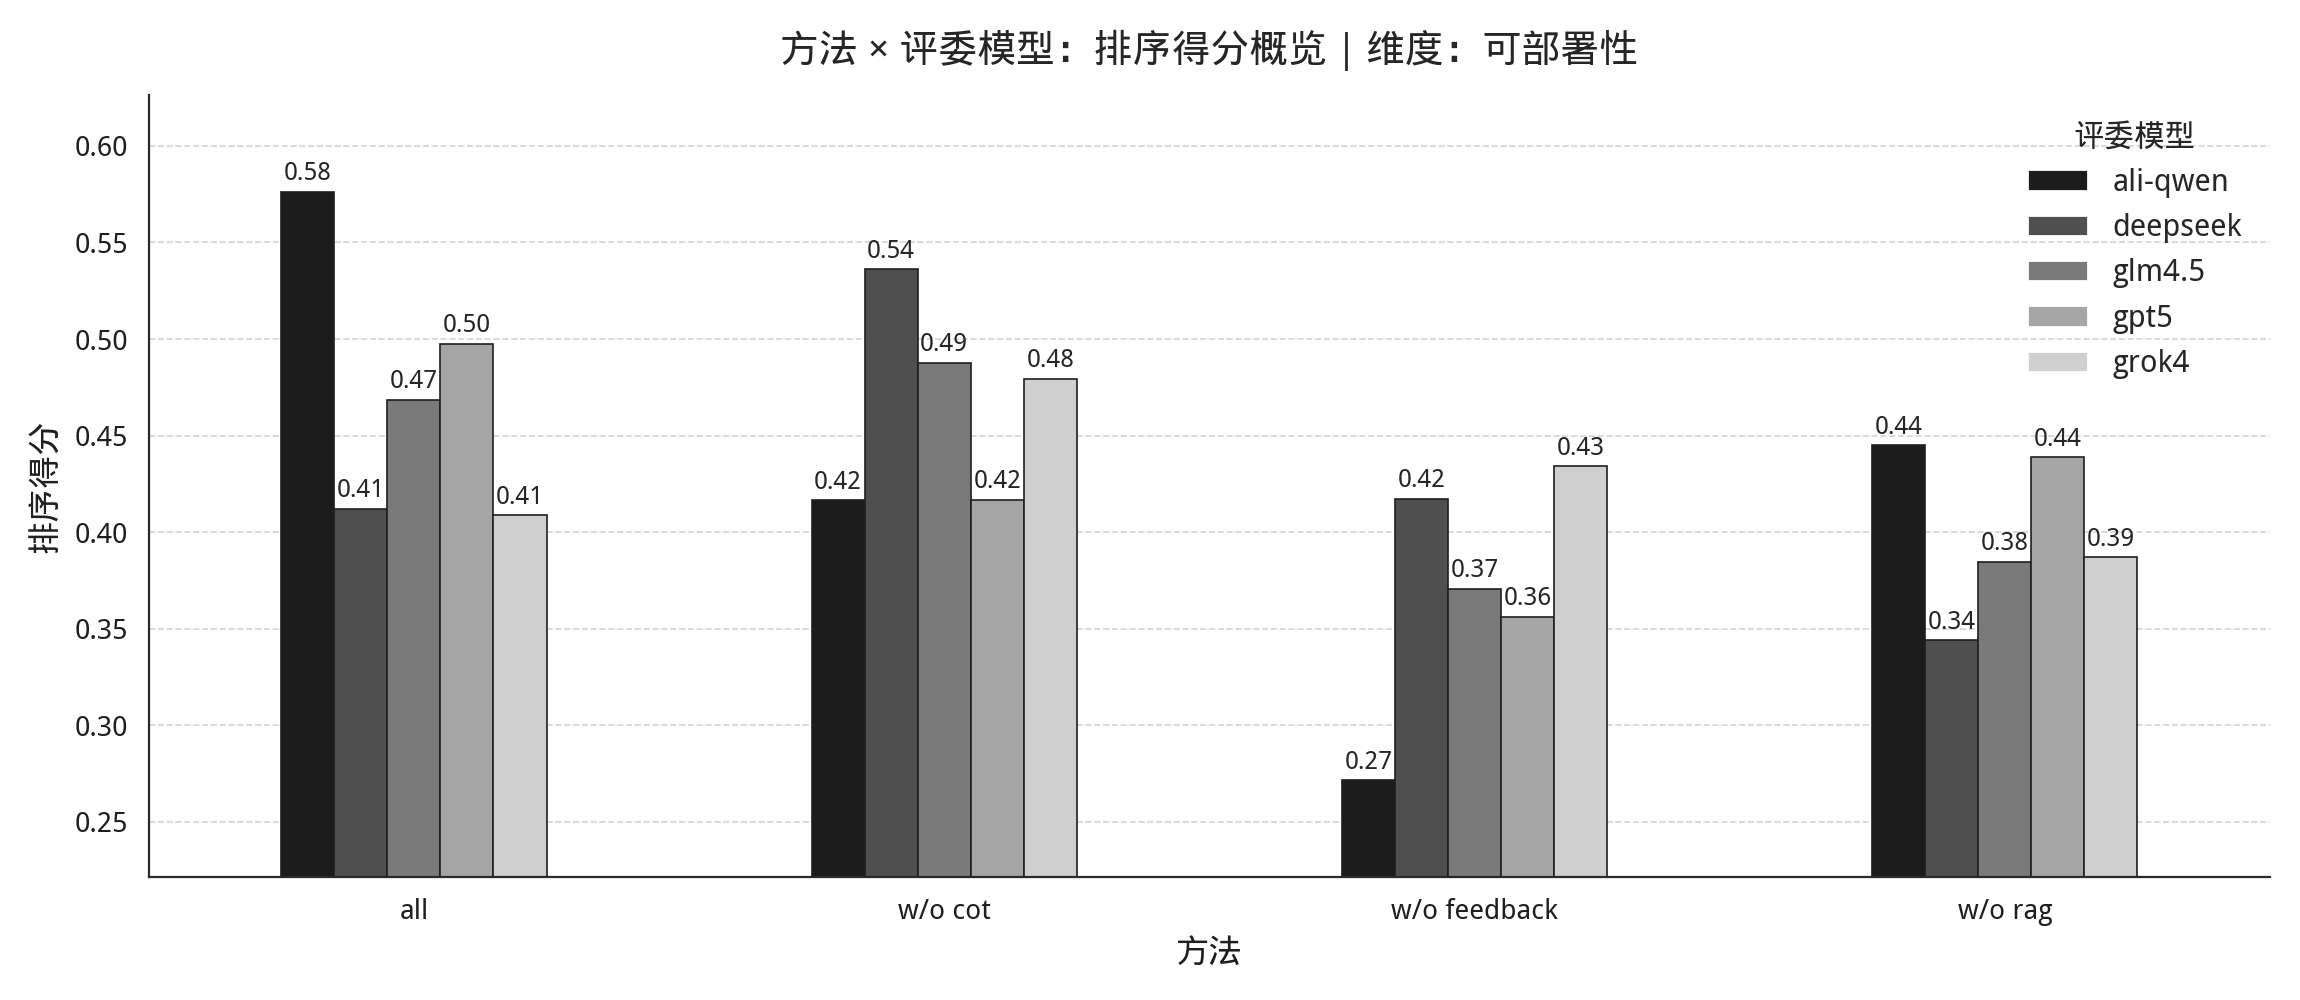
\includegraphics[width=0.32\textwidth]{images/plots/可部署性/summary/single_dim_by_judge_可部署性.png}}\hfill
	 \subfloat[无干扰性\label{fig:single-dim-interference}]{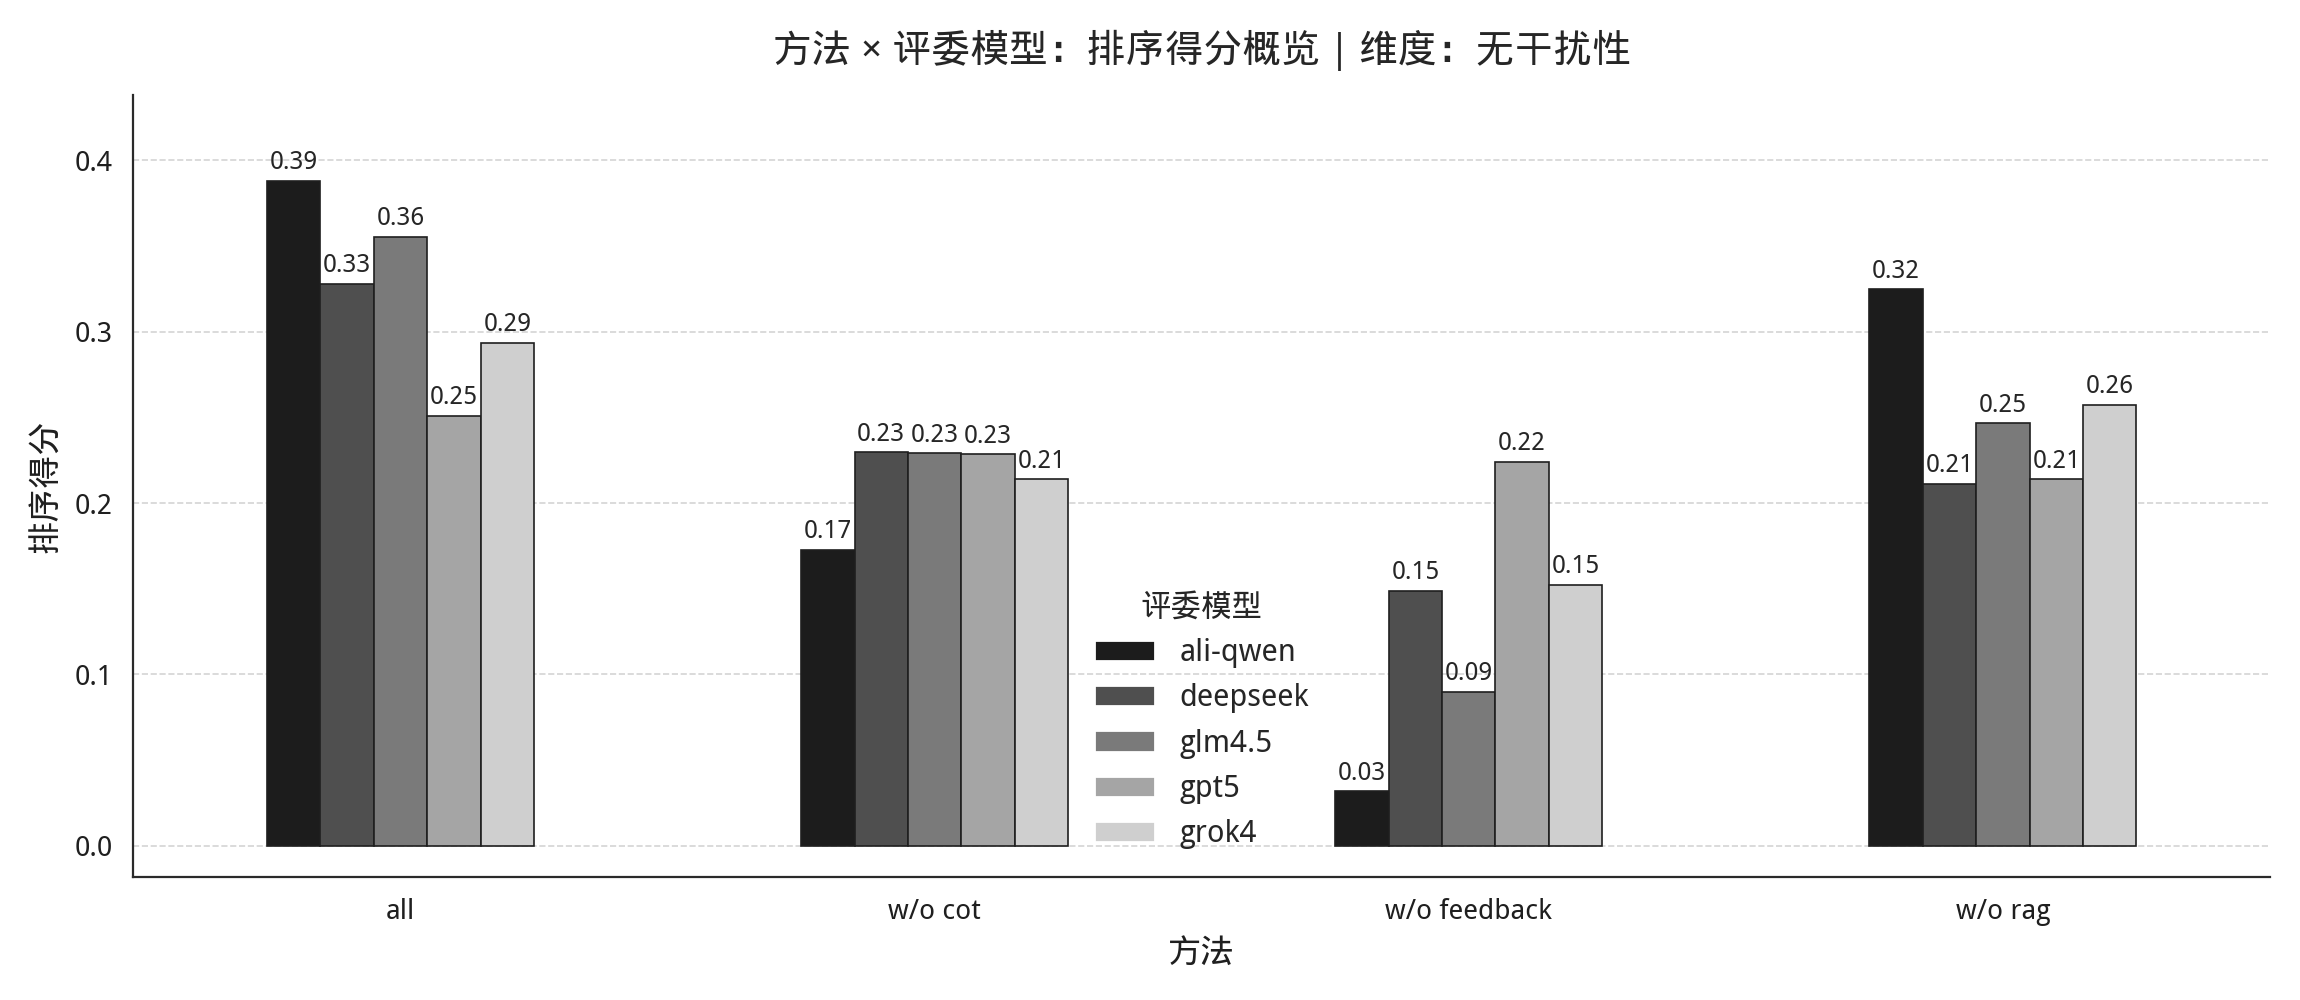
\includegraphics[width=0.32\textwidth]{images/plots/无干扰性/summary/single_dim_by_judge_无干扰性.png}}\hfill
	 \subfloat[有效性\label{fig:single-dim-effectiveness}]{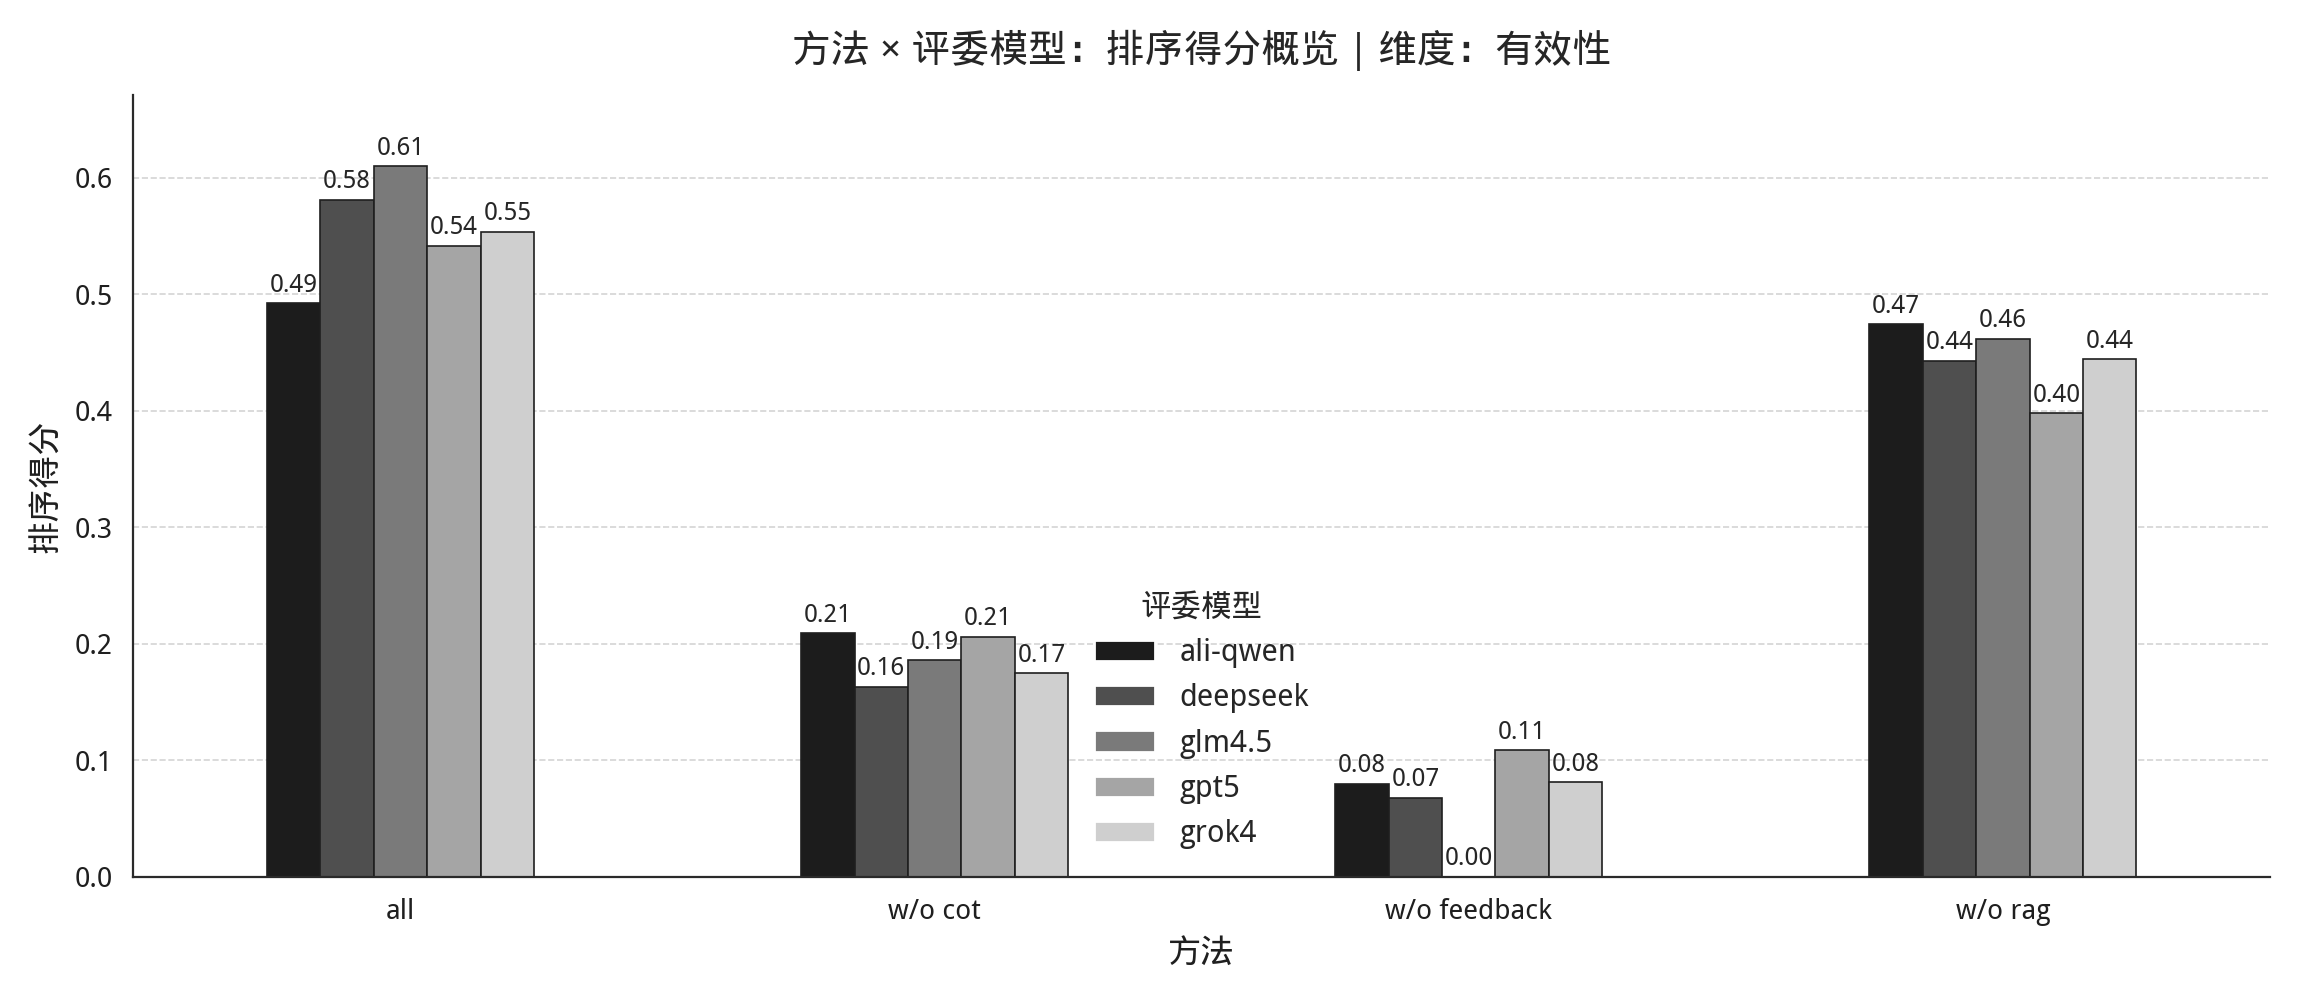
\includegraphics[width=0.32\textwidth]{images/plots/有效性/summary/single_dim_by_judge_有效性.png}}}
	\caption{不同评审模型下的单维度排名式评分结果（三维度并列）。}\label{fig:single-dim-by-judge-3d}
\end{figure}

\begin{figure}[!ht]
	\centering
	{\setlength{\abovecaptionskip}{2pt}%
	 \setlength{\belowcaptionskip}{0pt}%
	 \subfloat[可部署性\label{fig:single-dim-profile-avg-deployability}]{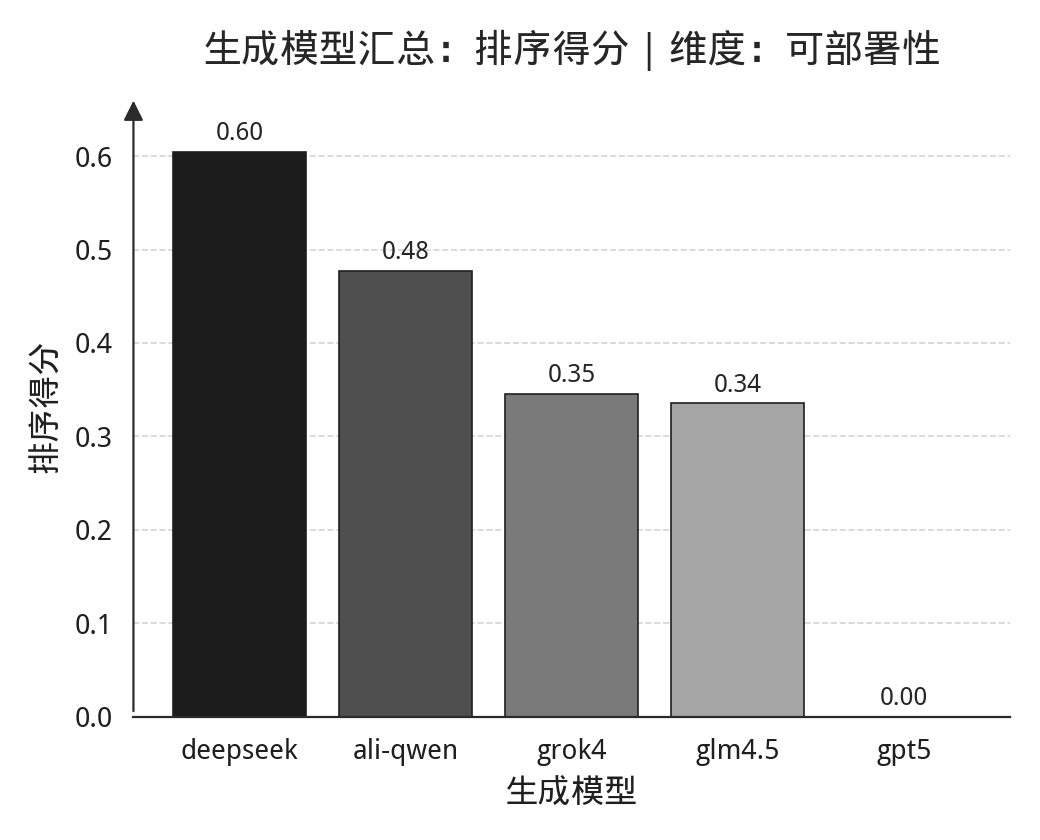
\includegraphics[width=0.32\textwidth]{images/plots/可部署性/summary/single_dim_profile_avg_可部署性.png}}\hfill
	 \subfloat[无干扰性\label{fig:single-dim-profile-avg-interference}]{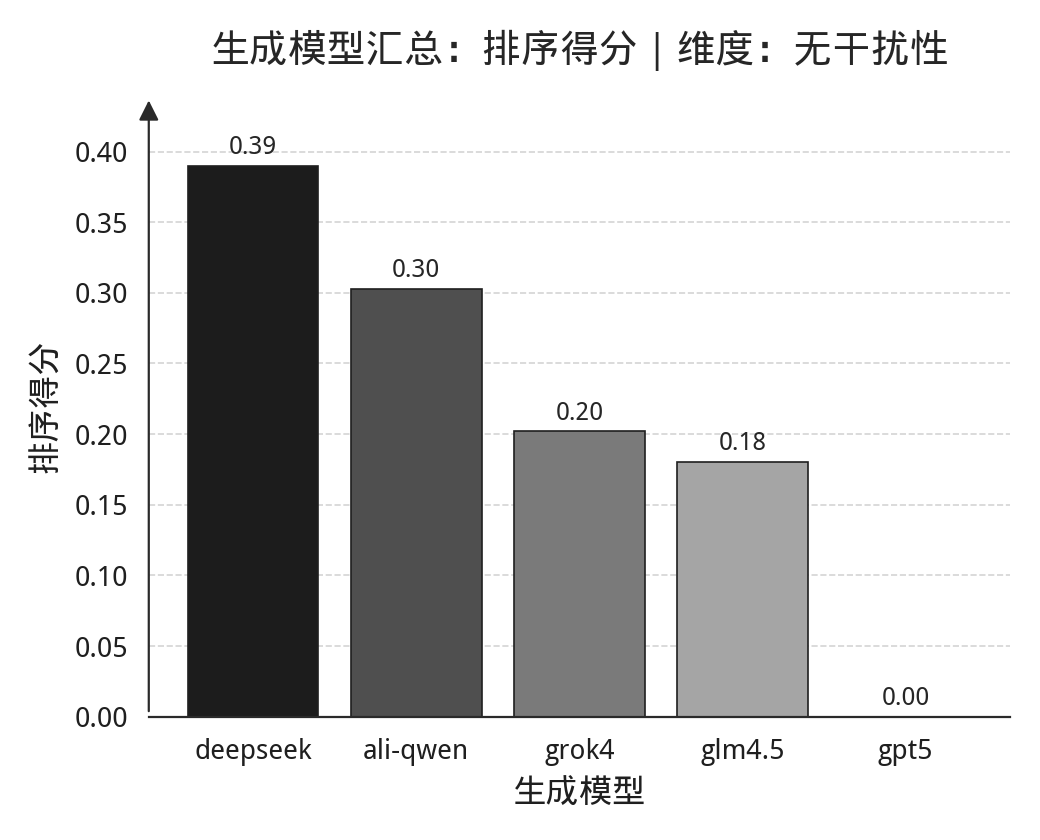
\includegraphics[width=0.32\textwidth]{images/plots/无干扰性/summary/single_dim_profile_avg_无干扰性.png}}\hfill
	 \subfloat[有效性\label{fig:single-dim-profile-avg-effectiveness}]{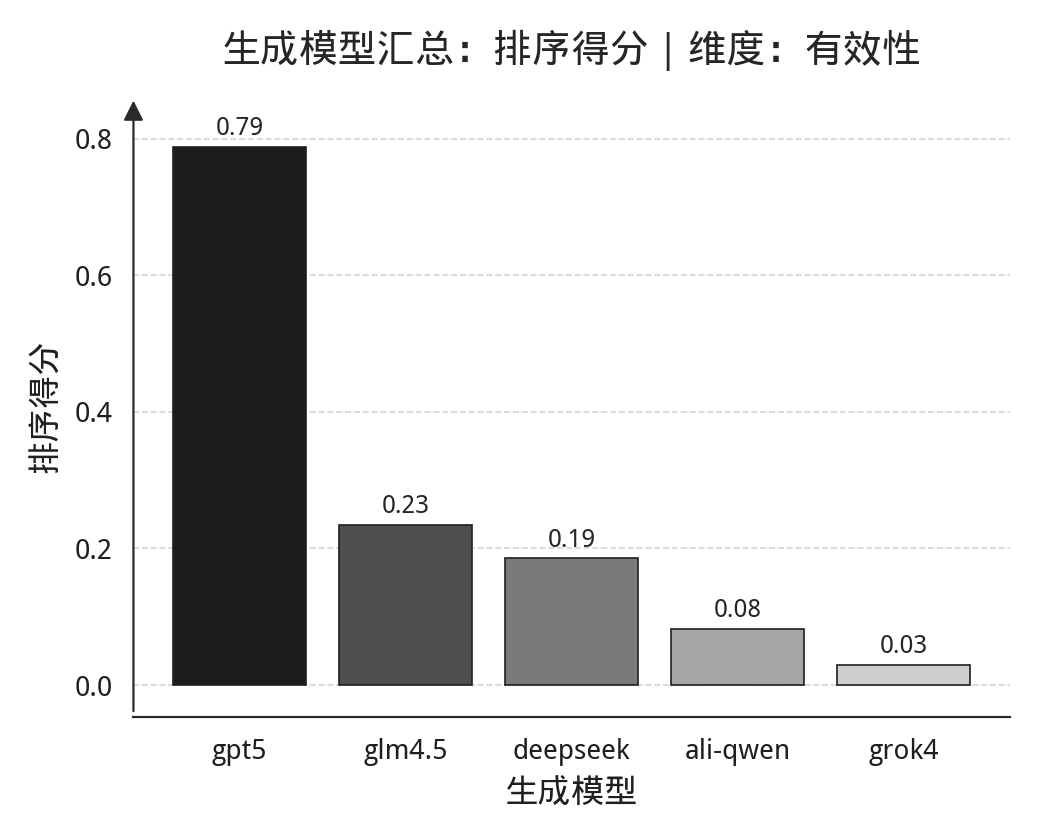
\includegraphics[width=0.32\textwidth]{images/plots/有效性/summary/single_dim_profile_avg_有效性.png}}}
	\caption{不同生成模型在三个维度上的平均排名式评分结果（跨评审者汇总，三维度并列）。}\label{fig:single-dim-profile-avg}
\end{figure}

\subsection{一致性度量与评审可信度}

为验证排名式评价的可信度，本小节分析不同评审模型在单一维度与跨维度场景下的一致性。若不同评审者（评审模型）对候选项优劣的判断高度一致，则聚合后的排序结果更稳定、更可解释；反之，若一致性较弱，则需要警惕"评审者选择敏感性"，并进一步细化评价准则。

在固定评价维度下，设共有 $n$ 个候选项（例如不同方法配置）与 $m$ 名评审者。候选项索引 $i=1,\dots,n$，评审者索引 $j=1,\dots,m$。令 $r_{ij}$ 表示评审者 $j$ 对候选项 $i$ 给出的名次（名次越小表示越优）。

\textbf{Kendall's $W$（协调系数）} 用于刻画多评审者整体一致性，取值范围 $[0,1]$，$W=1$ 表示完全一致：
\begin{equation}
W = \frac{12\,S}{m^2\,(n^3-n)}
\end{equation}
其中
\begin{equation}
S=\sum_{i=1}^{n}(R_i-\bar{R})^2,\quad R_i=\sum_{j=1}^{m} r_{ij},\quad \bar{R}=\frac{1}{n}\sum_{i=1}^{n}R_i.
\end{equation}

\textbf{两两 Spearman 等级相关系数} 用于刻画任意两名评审者排序趋势的一致性。对评审者 $j$ 与 $k$，其排名向量分别记为 $\mathbf{r}_j$ 与 $\mathbf{r}_k$，则
\begin{equation}
\rho_{jk}=\mathrm{corr}(\mathbf{r}_j,\mathbf{r}_k).
\end{equation}
当两位评审者排序趋势一致时，$\rho_{jk}$ 接近 $1$；当趋势相反时，$\rho_{jk}$ 接近 $-1$。

本文在 $E/I/D$ 三个维度内分别计算 Kendall's $W$ 与评审者两两 Spearman 相关系数，并汇总其分布统计。结果显示（见图\ref{fig:judge-corr-3d}--\ref{fig:judge-spearman-box}）：
\begin{itemize}
	\item \textbf{有效性}：一致性最高，$W=0.955$；Spearman 均值 $0.944$（中位数 $0.944$，最小 $0.904$，最大 $0.991$）。
	\item \textbf{无干扰性}：一致性较高，$W=0.846$；Spearman 均值 $0.808$（中位数 $0.839$，最小 $0.585$，最大 $0.932$）。
	\item \textbf{可部署性}：一致性相对较弱，$W=0.687$；Spearman 均值 $0.609$（中位数 $0.689$，最小 $0.238$，最大 $0.947$）。
\end{itemize}
总体结论为：一致性呈现“有效性 $>$ 无干扰性 $>$ 可部署性”的稳定梯度。

\begin{figure}[!ht]
	\centering
	{\setlength{\abovecaptionskip}{2pt}%
	 \setlength{\belowcaptionskip}{0pt}%
	 \subfloat[有效性\label{fig:judge-corr-eff}]{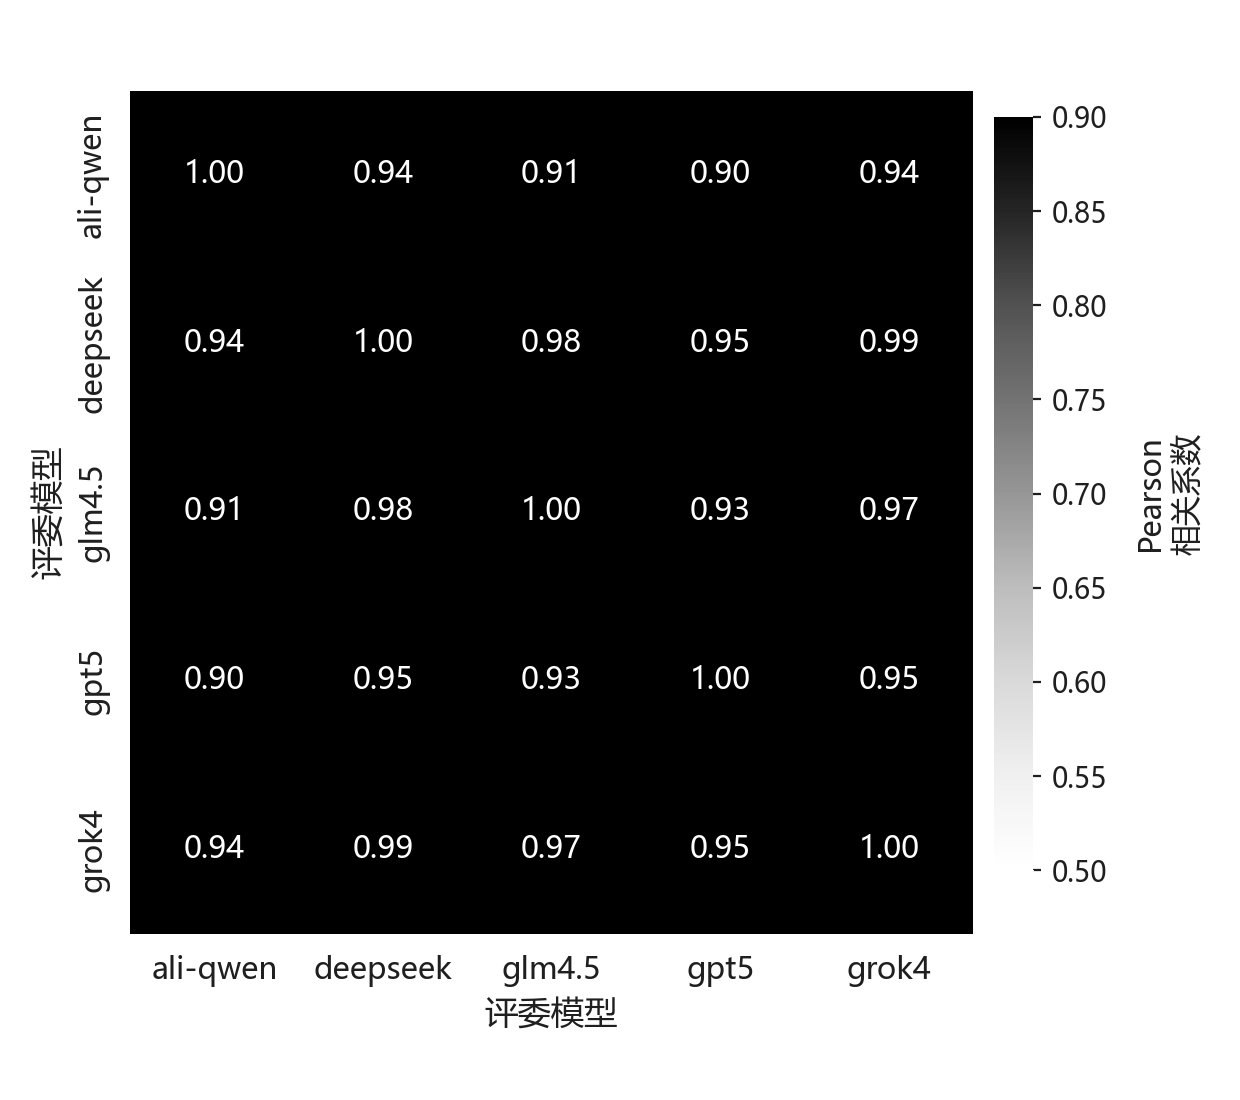
\includegraphics[width=0.32\textwidth]{images/plots/judge_consistency/judge_correlation_heatmap_有效性.png}}\hfill
	 \subfloat[无干扰性\label{fig:judge-corr-noint}]{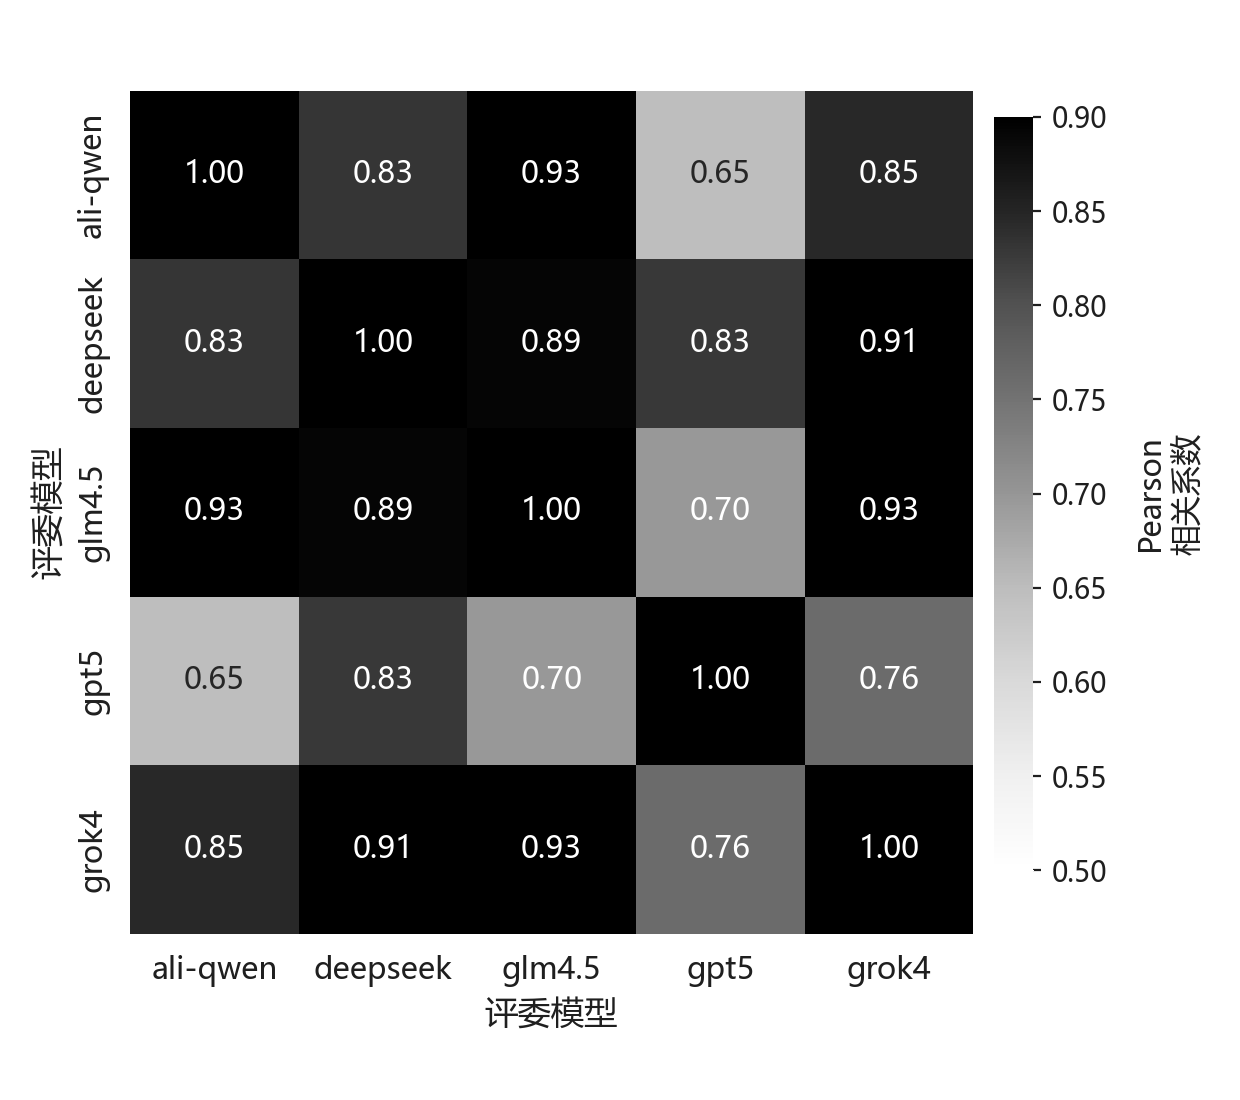
\includegraphics[width=0.32\textwidth]{images/plots/judge_consistency/judge_correlation_heatmap_无干扰性.png}}\hfill
	 \subfloat[可部署性\label{fig:judge-corr-deploy}]{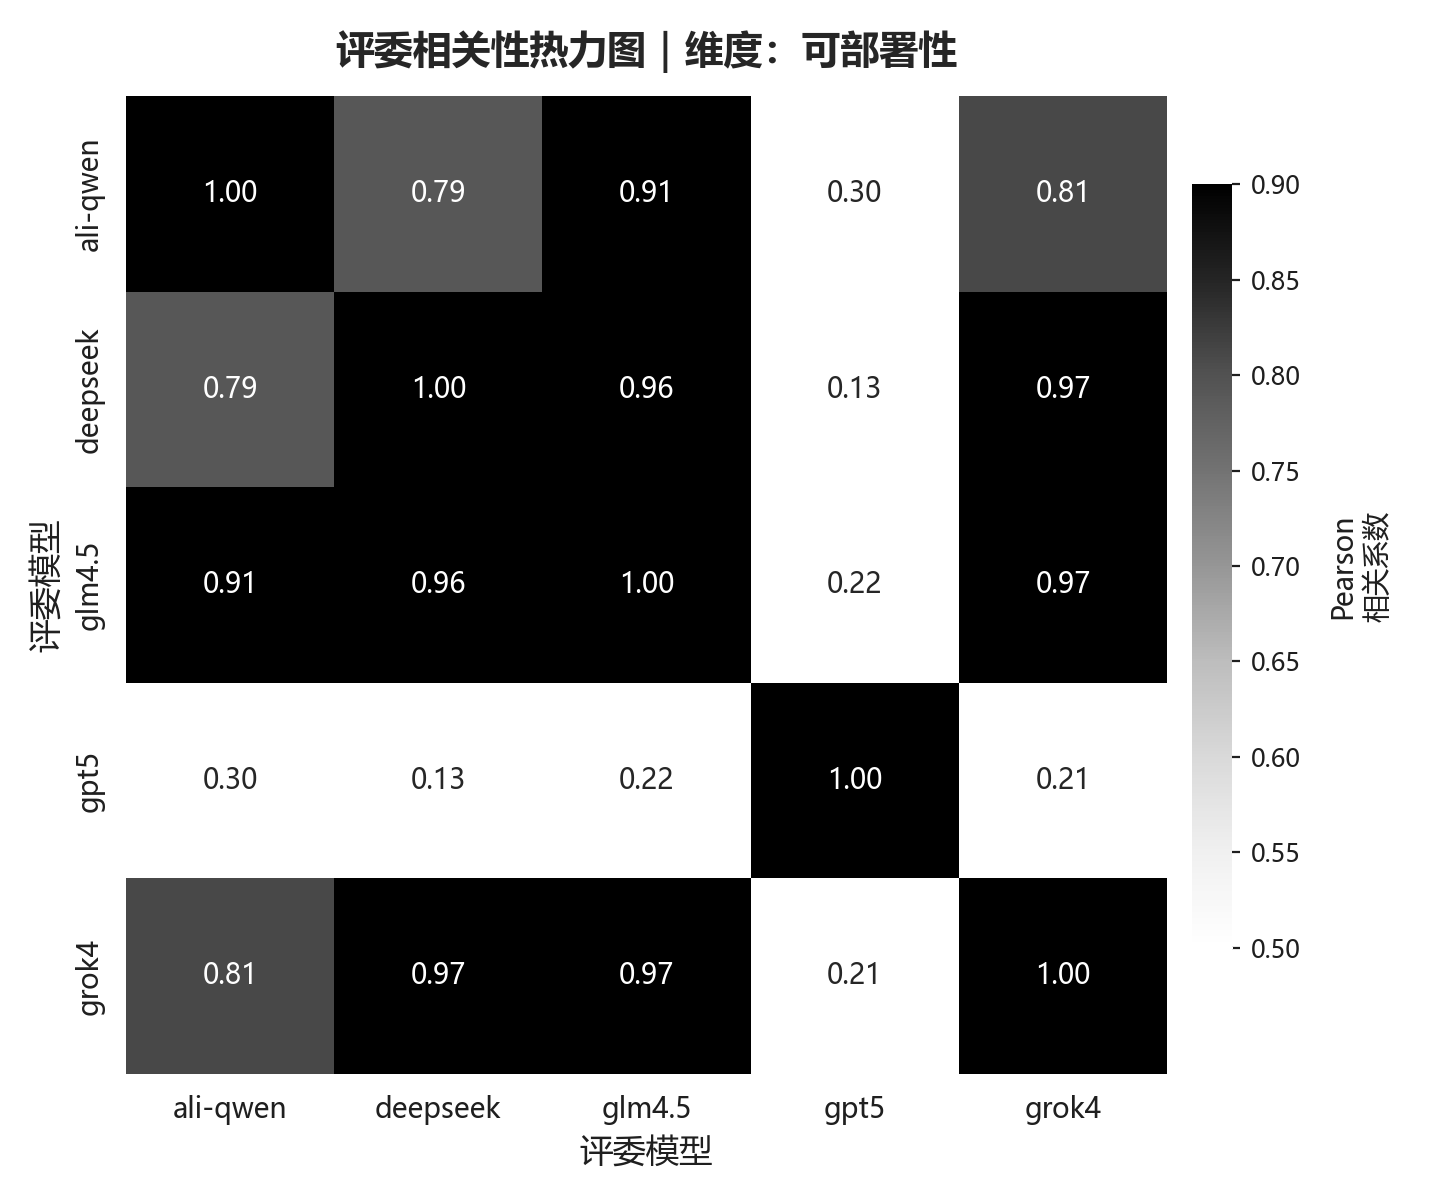
\includegraphics[width=0.32\textwidth]{images/plots/judge_consistency/judge_correlation_heatmap_可部署性.png}}}
	\caption{不同维度下评审者两两相关性热力图（Spearman）。}
	\label{fig:judge-corr-3d}
\end{figure}

\begin{figure}[!ht]
	\centering
	{\setlength{\abovecaptionskip}{2pt}%
	 \setlength{\belowcaptionskip}{0pt}%
	 \subfloat[Kendall's $W$ 对比\label{fig:judge-kendalls-w}]{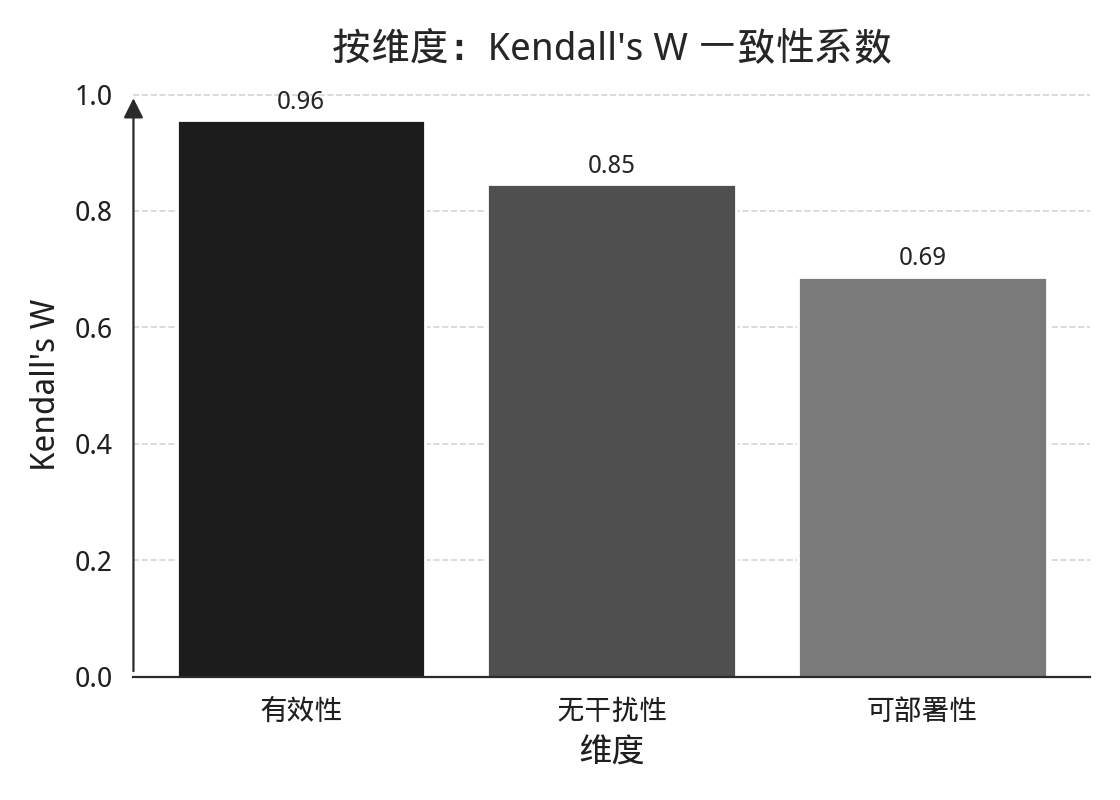
\includegraphics[width=0.49\textwidth]{images/plots/judge_consistency/judge_kendalls_w_by_dimension.png}}\hfill
	 \subfloat[两两 Spearman 分布\label{fig:judge-spearman-box}]{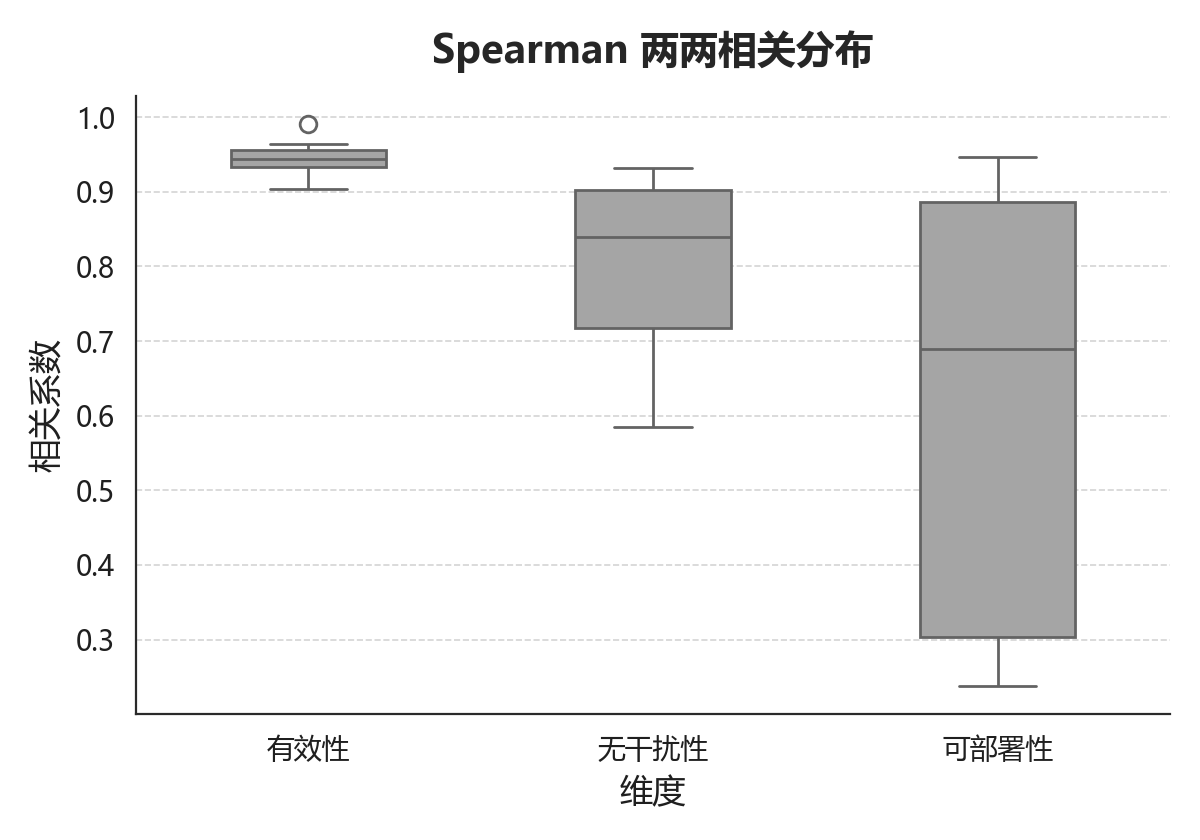
\includegraphics[width=0.49\textwidth]{images/plots/judge_consistency/judge_spearman_box_by_dimension.png}}}
	\caption{评审一致性统计汇总：整体一致性（$W$）与两两相关分布。}
	\label{fig:judge-agreement-summary}
\end{figure}

\begin{figure}[!ht]
	\centering
	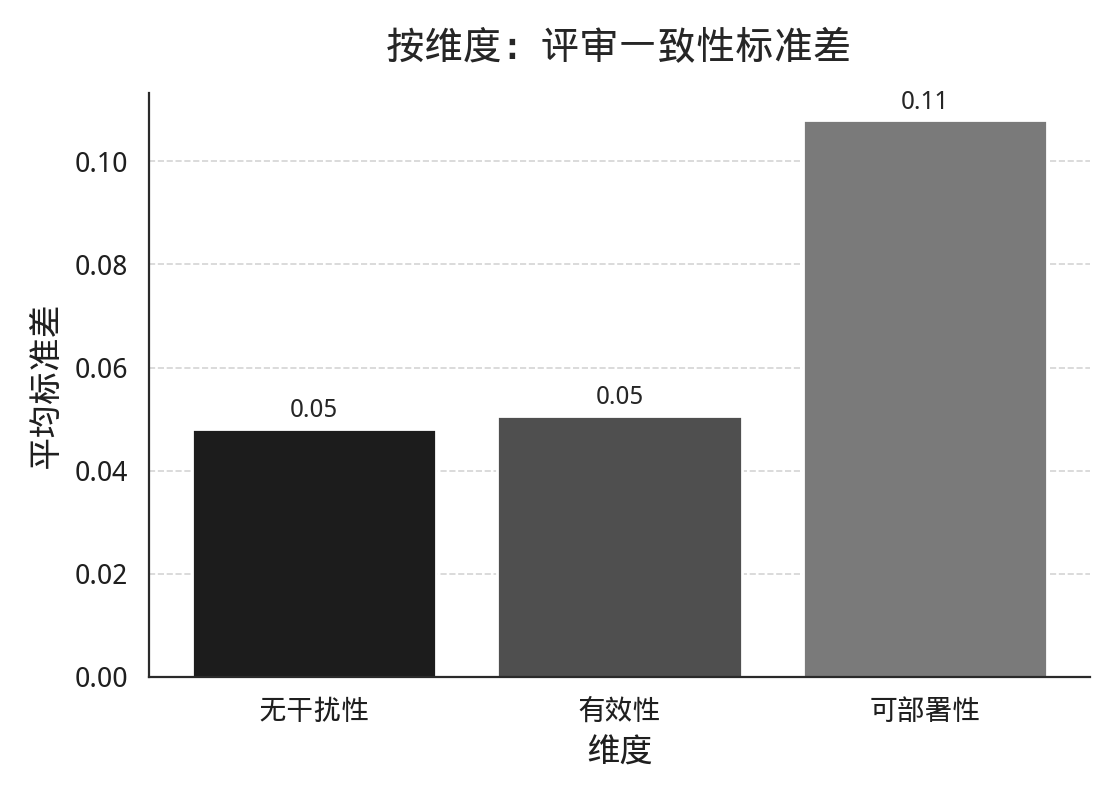
\includegraphics[width=0.86\linewidth]{images/plots/judge_consistency/judge_dispersion_by_dimension.png}
	\caption{不同维度下评审分歧程度的汇总（跨评审者离散性统计量）。}
	\label{fig:judge-dispersion}
\end{figure}

从一致性统计结果可以看出，不同评价维度下评审模型的一致性存在明显差异。有效性维度的一致性最高（$W=0.955$，Spearman均值$0.944$），说明评审者对"漏洞路径覆盖/处置有效性"的判定依据更为一致，这可能归因于有效性判定标准相对客观——漏洞是否被有效封堵、攻击路径是否被完全覆盖等技术指标具有较强的可验证性。相比之下，可部署性维度的一致性相对较弱（$W=0.687$，Spearman均值$0.609$），这与该维度涉及的评价因素更为复杂有关：工程可行性、环境依赖、部署成本与运维复杂度等多目标权衡使得不同评审者对权重与阈值的设定更易出现系统性差异。无干扰性维度的一致性则处于中间水平（$W=0.846$，Spearman均值$0.808$），反映了评审者在判断策略对业务流程影响时具有一定的共识基础，但仍存在因应用场景理解差异而产生的分歧。

尽管存在维度差异，较高的Kendall's $W$值与Spearman均值表明跨评审聚合后的排序整体稳定，足以为RQ1--RQ2的结论提供可信支撑。同时，对于一致性相对较弱的维度（如可部署性），后续可通过细化评价准则、增加典型案例边界说明，或采用鲁棒聚合策略（如中位数排名、加权投票等）来降低对单一评审者偏好的敏感性，进一步提升评价体系的稳定性与可解释性。



\section{RQ4：静态扫描的处置价值}

为评估静态扫描工具对临时防控决策的支撑程度，本文选取 \texttt{kubescape}、\texttt{kubesec} 与 \texttt{kubelinter} 作为代表性基线，并纳入 \texttt{SLI-Kube} 作为对照，在同一批 Kubernetes 清单上对报告条目按统一风险类型口径归并统计，结果如表\ref{tab:risk-summary-four-tools} 所示。整体上，静态工具的输出更偏向配置基线与通用加固项，适合用于日常治理与合规巡检；但从风险检测结果对具体 CVE 临时处置的直接支撑来看，其与本文统计的 55 个权限提升漏洞之间关联有限。对照分析显示，仅有 2 个漏洞样本 CVE\-2020\-4062 与 CVE\-2024\-31989 能在扫描报告中找到与触发前提一致的风险线索，且均属于缺乏网络隔离风险，对应表中的网络隔离项，分别由 \texttt{kubescape} 与 \texttt{SLI-Kube} 命中。除上述情形外，其余漏洞样本的关键攻击路径与触发条件通常未被静态扫描规则直接覆盖，难以在补丁窗口期形成可执行的处置依据。

\begin{table}[t]
\centering
\small
% 注：列类型 Y 已在本章前部定义（避免重复定义产生 warning）
% 将表格宽度设置为 \linewidth，第一列左对齐(l)，其余列均匀分布并居中(Y)
\bicaption{静态扫描工具风险结果汇总}{Summary of risk types from static scanning tools}
\begin{tabularx}{0.95\linewidth}{l *{5}{>{\centering\arraybackslash}X}}
\toprule
风险类型 & 关联一级分类 & Kubescape & Kubesec & Kubelinter & SLI-Kube\\
\midrule
资源配置缺失 & 配置缺陷 & 110 & 47 & 73 & 0 \\
非 Root 运行 & 配置缺陷 & 54 & 53 & 51 & 0 \\
根文件系统非只读 & 配置缺陷 & 39 & 34 & 59 & 0 \\
网络隔离 & 配置缺陷 & 132 & 0 & 0 & 15 \\
特权与提权 & 配置缺陷 & 39 & 0 & 12 & 0 \\
主机级暴露 & 配置缺陷 & 30 & 0 & 9 & 3 \\
身份与密钥 & 敏感信息泄露 & 192 & 58 & 0 & 2 \\
系统调用隔离 & 配置缺陷 & 0 & 58 & 0 & 1 \\
探针配置 & 配置缺陷 & 92 & 0 & 15 & 0 \\
\bottomrule
\end{tabularx}
\label{tab:risk-summary-four-tools}
\end{table}

\section{RQ5：资源消耗与效率评估}

资源消耗包括令牌消耗（token usage）与时间成本（elapsed time），共同构成生成式工作流在补丁窗口期及受限部署环境中的可用性约束。令牌消耗直接关联API调用的经济成本，而时间成本决定了在紧急漏洞响应场景下能否及时完成策略生成与评审闭环。本节旨在以严谨的计量口径刻画不同方法配置下的双维度资源消耗结构，并通过成本-收益分析判断在给定资源预算与时间约束下的最优折衷。

\subsection{令牌消耗统计}

下表展示不同方法配置与生成模型下的平均令牌消耗及对应的经济成本：

\begin{table}[htb]
\centering
% 注：列类型 Y 已在本章前部定义（避免重复定义产生 warning）

\bicaption{不同数据集与大模型下的平均Token消耗对比}{Comparison of average token usage across datasets and LLMs}
\label{tab:token_usage_wide}

% 设置行高与列间距
\renewcommand{\arraystretch}{1.15}
\setlength{\tabcolsep}{4pt}
\footnotesize

% 自动生成：Token/成本统计表格
% 依赖: \usepackage{booktabs} 以及 \usepackage{multirow}

\begin{tabular}{>{\raggedright\arraybackslash}p{2.0cm} >{\raggedright\arraybackslash}p{1.8cm} r r r r r r}
\toprule
\textbf{方法} & \textbf{模型} & \makecell{\textbf{输入}\\\textbf{Token}} & \makecell{\textbf{输出}\\\textbf{Token}} & \makecell{\textbf{输入成本}\\\textbf{(CNY)}} & \makecell{\textbf{输出成本}\\\textbf{(CNY)}} & \makecell{\textbf{总成本}\\\textbf{(CNY)}} & \makecell{\textbf{平均成本}\\\textbf{(CNY)}} \\ 
\midrule
\multirow{5}{*}{\texttt{All}} & ali-qwen & 228,842 & 92,360 & 0.57 & 0.92 & 1.50 & \multirow{5}{*}{12.99} \\ 
 & deepseek & 213,174 & 360,923 & 0.51 & 2.60 & 3.11 & \\ 
 & glm4.5 & 217,216 & 158,493 & 0.17 & 0.32 & 0.49 & \\ 
 & gpt5 & 376,812 & 672,931 & 3.30 & 47.11 & 50.40 & \\ 
 & grok4 & 246,549 & 108,188 & 2.96 & 6.49 & 9.45 & \\ 
\addlinespace[0.25em]\midrule
\multirow{5}{*}{\texttt{W/O CoT}} & ali-qwen & 147,128 & 44,759 & 0.37 & 0.45 & 0.82 & \multirow{5}{*}{11.29} \\ 
 & deepseek & 143,191 & 310,209 & 0.34 & 2.23 & 2.58 & \\ 
 & glm4.5 & 138,905 & 141,923 & 0.11 & 0.28 & 0.39 & \\ 
 & gpt5 & 201,623 & 646,417 & 1.76 & 45.25 & 47.01 & \\ 
 & grok4 & 165,321 & 61,481 & 1.98 & 3.69 & 5.67 & \\ 
\addlinespace[0.25em]\midrule
\multirow{5}{*}{\texttt{W/O Feedback}} & ali-qwen & 129,241 & 44,841 & 0.32 & 0.45 & 0.77 & \multirow{5}{*}{9.88} \\ 
 & deepseek & 120,138 & 280,609 & 0.29 & 2.02 & 2.31 & \\ 
 & glm4.5 & 122,551 & 155,095 & 0.10 & 0.31 & 0.41 & \\ 
 & gpt5 & 178,449 & 554,871 & 1.56 & 38.84 & 40.40 & \\ 
 & grok4 & 145,538 & 62,736 & 1.75 & 3.76 & 5.51 & \\ 
\addlinespace[0.25em]\midrule
\multirow{5}{*}{\texttt{W/O RAG}} & ali-qwen & 184,820 & 46,291 & 0.46 & 0.46 & 0.92 & \multirow{5}{*}{11.10} \\ 
 & deepseek & 170,295 & 318,002 & 0.41 & 2.29 & 2.70 & \\ 
 & glm4.5 & 170,290 & 116,108 & 0.14 & 0.23 & 0.37 & \\ 
 & gpt5 & 338,456 & 603,583 & 2.96 & 42.25 & 45.21 & \\ 
 & grok4 & 203,726 & 64,326 & 2.44 & 3.86 & 6.30 & \\ 
\addlinespace[0.25em]
\bottomrule
\end{tabular}
\end{table}

\subsection{时间成本统计}

时间成本直接影响在紧急漏洞响应场景下的可用性。下表统计了56个CVE样本在不同方法配置与生成模型下的总耗时与平均耗时（单位：秒）：

\begin{table}[htb]
\centering
\bicaption{不同方法配置与生成模型下的时间成本统计}{Time cost statistics across method configurations and LLMs}
\label{tab:time_cost}

\renewcommand{\arraystretch}{1.15}
\setlength{\tabcolsep}{5pt}
\footnotesize

\begin{tabular}{>{\raggedright\arraybackslash}p{2.2cm} >{\raggedright\arraybackslash}p{1.8cm} r r r}
\toprule
\textbf{方法配置} & \textbf{模型} & \makecell{\textbf{总耗时}\\\textbf{(秒)}} & \makecell{\textbf{平均耗时}\\\textbf{(秒)}} & \makecell{\textbf{CVE}\\\textbf{数量}} \\ 
\midrule
\multirow{5}{*}{\texttt{All}} & ali-qwen & 1,543.84 & 27.57 & 56 \\ 
 & deepseek & 11,918.95 & 212.84 & 56 \\ 
 & glm4.5 & 3,098.98 & 55.34 & 56 \\ 
 & gpt5 & 19,063.76 & 340.42 & 56 \\ 
 & grok4 & 1,469.06 & 26.23 & 56 \\ 
\addlinespace[0.25em]\midrule
\multirow{5}{*}{\texttt{W/O CoT}} & ali-qwen & 1,468.46 & 26.22 & 56 \\ 
 & deepseek & 12,283.19 & 219.34 & 56 \\ 
 & glm4.5 & 4,156.38 & 74.22 & 56 \\ 
 & gpt5 & 18,394.20 & 328.47 & 56 \\ 
 & grok4 & 1,675.92 & 29.93 & 56 \\ 
\addlinespace[0.25em]\midrule
\multirow{5}{*}{\texttt{W/O Feedback}} & ali-qwen & 0.00 & 0.00 & 56 \\ 
 & deepseek & 0.00 & 0.00 & 56 \\ 
 & glm4.5 & 0.00 & 0.00 & 56 \\ 
 & gpt5 & 0.00 & 0.00 & 56 \\ 
 & grok4 & 0.00 & 0.00 & 56 \\ 
\addlinespace[0.25em]\midrule
\multirow{5}{*}{\texttt{W/O RAG}} & ali-qwen & 1,620.01 & 28.93 & 56 \\ 
 & deepseek & 12,051.22 & 215.20 & 56 \\ 
 & glm4.5 & 3,683.49 & 65.78 & 56 \\ 
 & gpt5 & 19,290.87 & 344.48 & 56 \\ 
 & grok4 & 1,542.77 & 27.55 & 56 \\ 
\addlinespace[0.25em]
\bottomrule
\end{tabular}
\end{table}

\subsection{综合分析与折衷策略}

从时间成本角度观察：
\begin{itemize}
	\item \textbf{快速响应型}：\texttt{Grok4} 与 \texttt{ali-qwen} 在完整配置（All）下平均耗时仅26--28秒/样本，适合紧急漏洞响应场景。
	\item \textbf{高精度型}：\texttt{GPT-5} 与 \texttt{DeepSeek} 平均耗时显著较高（212--340秒/样本），但在有效性与可部署性维度表现优异（见RQ2），适合非紧急场景下的高质量策略生成。
	\item \textbf{反馈闭环的时间开销}：W/O Feedback配置下所有模型耗时为0，反映反馈闭环在时间维度的显著贡献；完整配置下反馈闭环带来的额外耗时在GPT-5上最为明显（340秒），但同时也带来了有效性维度的最高得分（0.814，见表\ref{tab:generator-scores}）。
\end{itemize}

结合令牌成本与时间成本的双维度权衡：
\begin{itemize}
	\item 在\textbf{资源与时间双约束}场景下，\texttt{ali-qwen}（完整配置）表现出最优的成本-效益比：经济成本1.50元、平均耗时27.57秒，同时在无干扰性与可部署性维度保持中等水平。
	\item 在\textbf{追求极致性能}场景下，\texttt{GPT-5}（完整配置）以50.40元经济成本与340.42秒耗时为代价，在有效性维度达到0.814的最高得分，适合高危漏洞的临时防控。
	\item 在\textbf{大规模批量处理}场景下，\texttt{DeepSeek} 提供了折衷方案：经济成本3.11元、平均耗时212.84秒，在可部署性维度表现优异（0.605），适合需要快速部署的中等风险漏洞。
\end{itemize}
